\documentclass[12pt,a4paper]{article}
\usepackage{fix-cm}
\usepackage{fontspec}
\setmainfont{Times New Roman}
\setsansfont{Times New Roman}
\setmonofont{Times New Roman}
\usepackage[vietnamese]{babel}
\usepackage[left=2.5cm,right=2cm,top=2cm,bottom=2cm]{geometry}
\usepackage{graphicx,booktabs,array,amsmath,amssymb}
\usepackage[authoryear,round]{natbib}
\usepackage{titlesec}
\let\cite\citep
\usepackage[hidelinks,unicode]{hyperref}
\hypersetup{pdftitle={FIT4013 – Đề tài 16: Dự đoán nguy cơ giao trễ},pdfauthor={Vũ Quốc Đoàn; Trần Đại Hiệp}}
\linespread{1}
\setlength{\parskip}{3pt}
\setlength{\parindent}{1.2em}
\setlength{\emergencystretch}{3em}
\setcounter{tocdepth}{2}
\renewcommand{\UrlFont}{\normalfont\rmfamily\fontsize{13bp}{15.6bp}\selectfont}
\newcommand{\code}[1]{\nolinkurl{#1}}
\newcommand{\fig}[4][.80]{\begin{figure}[!htbp]\centering
\includegraphics[width=#1\textwidth,height=.34\textheight,keepaspectratio]{../results/figures/#2}
\caption{#3}\label{#4}\end{figure}}
\ExplSyntaxOn
\NewExpandableDocumentCommand{\reportuppercase}{m}{\text_uppercase:n{#1}}
\ExplSyntaxOff
\newcommand{\partstart}[1]{\clearpage\section{\reportuppercase{#1}}\label{chap:\thesection}}
\begin{document}
\renewcommand{\contentsname}{MỤC LỤC}
\renewcommand{\refname}{TÀI LIỆU THAM KHẢO}
\renewcommand{\listfigurename}{DANH MỤC HÌNH ẢNH}
\renewcommand{\listtablename}{DANH MỤC BẢNG BIỂU}
% Only the first two pages of the supplied Word are used as cover references.
% bp = Word/PDF points (72/in): exported text is exactly 14 or 15 points.
\newcommand{\covertext}{\normalfont\rmfamily\fontsize{14bp}{17bp}\selectfont}
\newcommand{\covertitle}[1]{{\normalfont\rmfamily\fontsize{15bp}{18bp}\selectfont\bfseries #1\par}}
\newcommand{\coverblock}[4]{\put(#1,-#2){\makebox(0,0)[lt]{%
\begin{minipage}[t]{#3mm}\covertext\setlength{\parskip}{0pt}%
\centering #4\end{minipage}}}}
\newcommand{\coverframe}[3]{\AddToHookNext{shipout/background}{%
\setlength{\unitlength}{1mm}% x, bottom, height from Word's page rectangles.
\linethickness{2.2pt}\put(#1,-#2){\framebox(159,#3){}}%
\linethickness{.5pt}%
\put(\dimexpr#1mm+1mm\relax,\dimexpr-#2mm+1mm\relax){%
\framebox(157,\dimexpr#3mm-2mm\relax){}}}}
\newcommand{\topic}{\covertitle{DỰ ĐOÁN ĐƠN HÀNG CÓ NGUY CƠ\\
GIAO TRỄ TRONG CHUỖI CUNG ỨNG}}
\begin{titlepage}\thispagestyle{empty}\null
\coverframe{22.5}{278.1}{260.1}
\AddToHookNext{shipout/foreground}{\setlength{\unitlength}{1mm}%
\coverblock{31}{27.5}{153}{\covertitle{TRƯỜNG ĐẠI HỌC ĐẠI NAM}}
\coverblock{31}{33.6}{153}{\covertitle{KHOA CÔNG NGHỆ THÔNG TIN}}
\put(74.2,-39.5){\line(1,0){66.7}}
\put(76.5,-100.7){
\includegraphics[height=62mm]{assets/dainam_logo.png}}
\coverblock{31}{108}{153}{\covertitle{BÁO CÁO HỌC PHẦN}}
\coverblock{31}{124}{153}{\covertitle{NHẬP MÔN HỌC MÁY — FIT4013}}
\coverblock{31}{135}{153}{\covertitle{ĐỀ TÀI 16}}
\coverblock{31}{145}{153}{\topic}
\coverblock{47}{174}{135}{%
\begin{tabular}{@{}>{\raggedright\arraybackslash}p{5cm}>{\raggedright\arraybackslash}p{7.7cm}@{}}
Giảng viên hướng dẫn: & ThS. Lê Thị Thùy Trang\\[7pt]
Sinh viên thực hiện: & Vũ Quốc Đoàn — MSV: 1871020143\\[5pt]
 & Trần Đại Hiệp — MSV: 1871020223\\[7pt]
Lớp: & CNTT18-10\\[4pt]
Khóa: & K18\\[4pt]
Năm học: & 2026–2027
\end{tabular}}
\coverblock{31}{266}{153}{Hà Nội, 2026}}
\end{titlepage}
\begin{titlepage}\thispagestyle{empty}\null
\coverframe{28.55}{275.5}{257.4}
\AddToHookNext{shipout/foreground}{\setlength{\unitlength}{1mm}%
\coverblock{31}{31.3}{153}{\covertitle{TRƯỜNG ĐẠI HỌC ĐẠI NAM}}
\coverblock{31}{43.1}{153}{\covertitle{KHOA CÔNG NGHỆ THÔNG TIN}}
% Display rectangle follows Word page 2; the original logo bytes are unchanged.
\put(70.35,-99.7){
\includegraphics[width=74.3mm,height=46.5mm]{assets/dainam_logo.png}}
\coverblock{31}{106}{153}{\covertitle{BÁO CÁO HỌC PHẦN}}
\coverblock{31}{121}{153}{\covertitle{NHẬP MÔN HỌC MÁY — FIT4013}}
\coverblock{31}{134}{153}{\covertitle{ĐỀ TÀI 16}}
\coverblock{31}{146}{153}{\topic}
\coverblock{34}{185}{147}{%
\renewcommand{\arraystretch}{1.15}%
\begin{tabular}{|>{\raggedright\arraybackslash}p{5cm}|>{\raggedright\arraybackslash}p{8.6cm}|}\hline
\textbf{Hạng mục} & \textbf{Thông tin}\\\hline
Sinh viên / Nhóm & Vũ Quốc Đoàn — MSV: 1871020143\newline
Trần Đại Hiệp — MSV: 1871020223\\\hline
Lớp & CNTT18-10\\\hline
Khóa & K18\\\hline
Giảng viên hướng dẫn & ThS. Lê Thị Thùy Trang\\\hline
Năm học & 2026–2027\\\hline
\end{tabular}}
\coverblock{31}{248}{153}{Hà Nội, 2026}}
\end{titlepage}

% Body text, tables and captions: 13 Word/PDF points. Headings: 14/13/13.
% Local to the report body: cover.tex defines independent 14/15-point styles.
\makeatletter
\renewcommand\normalsize{\@setfontsize\normalsize{13bp}{15.6bp}%
  \abovedisplayskip 10pt plus 2pt minus 5pt
  \abovedisplayshortskip 0pt plus 3pt
  \belowdisplayshortskip 6pt plus 3pt minus 3pt
  \belowdisplayskip \abovedisplayskip}
\renewcommand\small{\normalsize}
\renewcommand\footnotesize{\normalsize}
\renewcommand\section{\@startsection{section}{1}{\z@}%
  {-3ex \@plus -1ex \@minus -.2ex}{1.75ex \@plus .2ex}%
  {\normalfont\fontsize{14bp}{16.8bp}\selectfont\bfseries}}
\renewcommand\subsection{\@startsection{subsection}{2}{\z@}%
  {-2.5ex \@plus -1ex \@minus -.2ex}{1.25ex \@plus .2ex}%
  {\normalfont\fontsize{13bp}{15.6bp}\selectfont\bfseries}}
\renewcommand\subsubsection{\@startsection{subsubsection}{3}{\z@}%
  {-2.5ex \@plus -1ex \@minus -.2ex}{1.25ex \@plus .2ex}%
  {\normalfont\fontsize{13bp}{15.6bp}\selectfont\bfseries\itshape}}
\let\reportarrayparboxrestore\@arrayparboxrestore
\def\@arrayparboxrestore{\reportarrayparboxrestore\raggedright\arraybackslash}
\makeatother
\normalsize

\pagenumbering{roman}
\phantomsection
\section*{LỜI MỞ ĐẦU}
\addcontentsline{toc}{section}{LỜI MỞ ĐẦU}
Giao hàng đúng hẹn là một yêu cầu quan trọng trong chuỗi cung ứng. Việc
nhận diện sớm đơn có nguy cơ giao trễ có thể hỗ trợ theo dõi và phân bổ
nguồn lực, nhưng cảnh báo sai hoặc bỏ sót đều cần được xem xét. Từ bối
cảnh đó, nhóm lựa chọn đề tài dự đoán nguy cơ giao trễ để vận dụng kiến
thức học phần vào một bài toán phân loại dữ liệu bảng.

Báo cáo sử dụng DataCo Smart Supply Chain, với K-Nearest Neighbors và
Decision Tree là hai thuật toán chính. Quy trình gồm kiểm toán dữ liệu,
lựa chọn đặc trưng, tiền xử lý, chia nhóm theo mã đơn, kiểm định chéo và
đánh giá. Hai luồng A/B cùng các baseline được đối chiếu bằng kết quả
đã lưu trong repository. Các kết luận phân biệt rõ dòng hàng với đơn
hàng và giới hạn của tập con thực nghiệm, không suy rộng thành hiệu quả
vận hành đã được chứng minh.

Báo cáo gồm sáu chương theo thứ tự: đặt vấn đề và phân tích yêu cầu;
thiết kế giải pháp; phân tích mã nguồn; thử nghiệm và kết quả; thảo luận
và so sánh; tổng kết và hướng phát triển.

\phantomsection
\section*{PHÂN CÔNG NHIỆM VỤ}
\addcontentsline{toc}{section}{PHÂN CÔNG NHIỆM VỤ}
\begin{table}[!htbp]\centering\small
\caption{Phân công nhiệm vụ dự kiến, chờ hai thành viên xác nhận.}\label{tab:team-assignment}
\begin{tabularx}{\linewidth}{p{3.6cm}Y}\toprule
\rowcolor{reportheader} \theadcell{Họ tên thành viên} & \theadcell{Nhiệm vụ được phân công}\\\midrule
Vũ Quốc Đoàn\newline 1871020143 & Nghiên cứu bài toán, dataset; phân tích EDA; tiền xử lý và lựa chọn đặc trưng; phân tích luồng A/B; tham gia hoàn thiện báo cáo.\\[7pt]
Trần Đại Hiệp\newline 1871020223 & Nghiên cứu K-NN và Decision Tree; xây dựng pipeline huấn luyện; cross-validation và đánh giá; phân tích kết quả, ma trận nhầm lẫn và lỗi; tham gia hoàn thiện báo cáo.\\\bottomrule
\end{tabularx}
\end{table}

\clearpage\pdfbookmark[1]{MỤC LỤC}{report-toc}\tableofcontents
\clearpage\phantomsection
\addcontentsline{toc}{section}{DANH MỤC HÌNH ẢNH}
\listoffigures
\phantomsection
\addcontentsline{toc}{section}{DANH MỤC BẢNG BIỂU}
\listoftables
\clearpage\pagenumbering{arabic}
\partstart{Đặt vấn đề và phân tích yêu cầu}
\subsection{Bối cảnh và động cơ nghiên cứu}
Trong chuỗi cung ứng, một đơn hàng đi qua nhiều bước từ tiếp nhận, chuẩn bị
hàng, lựa chọn phương thức vận chuyển đến giao cho khách. Nếu chỉ phát hiện
chậm giao khi đã vượt thời hạn cam kết, cơ hội điều phối sớm bị thu hẹp.
Bài toán của đề tài 16 vì vậy tập trung vào cảnh báo nguy cơ: sử dụng các
thuộc tính có thể biết khi tạo đơn để nhận diện những đơn cần được theo dõi.
Kết quả phân loại có thể là đầu vào cho nhân viên vận hành xem xét, thay vì
tự động thay đổi cam kết giao hàng.

Một cảnh báo đúng có thể hỗ trợ ưu tiên kiểm tra tồn kho hoặc rà soát kế
hoạch vận chuyển. Ngược lại, cảnh báo sai gây thêm khối lượng xử lý, còn bỏ
sót khiến đơn có vấn đề không được chú ý. Báo cáo không gán giá trị tiền cho
những tác động này vì dữ liệu hiện có không chứa chi phí can thiệp. Sự hữu
ích của cảnh báo phải được đánh giá cùng khả năng xử lý của đơn vị vận hành,
không thể suy ra chỉ từ độ chính xác của mô hình.

Đề tài phù hợp với dữ liệu bảng có cả số và phân loại. K-NN được chọn để
khảo sát việc dự đoán từ những đơn có đặc trưng tương tự; cây quyết định
được chọn để khảo sát quy tắc chia nhóm. Hai thuật toán có cách biểu diễn
ranh giới khác nhau, tạo cơ sở so sánh giữa học dựa trên khoảng cách và học
dựa trên các điều kiện phân nhánh. Đây cũng là hai phương pháp thuộc phạm
vi thuật toán học phần quy định \cite{fit}.

\subsection{Mục tiêu, thời điểm dự đoán và phạm vi}
Biến mục tiêu là \code{Late_delivery_risk}, nhận giá trị 1 nếu nguồn gán
nguy cơ giao trễ, và 0 cho phần còn lại. Bài toán được phát biểu dưới dạng
học có giám sát: từ vector đặc trưng $x_i$ của một dòng hàng, ước lượng nhãn
$\hat y_i\in\{0,1\}$. Mỗi dòng còn gắn với một mã đơn $g_i$; các dòng chung
mã đơn có thể dùng chung phương thức vận chuyển và thông tin khách hàng.

Thời điểm dự đoán giả định là sau khi đơn được tạo và phương thức giao đã
được chọn, trước ngày vận chuyển và kết quả giao thực tế. Giả định này quyết
định các trường được phép làm đầu vào. Nếu doanh nghiệp muốn dự đoán trước
cả bước lựa chọn phương thức giao, danh sách đặc trưng hiện tại không còn
phù hợp và phải thiết kế lại bài toán. Tính sẵn có của từng trường cần được
chủ dữ liệu xác nhận trước ứng dụng.

Mục tiêu thực nghiệm gồm xây dựng quy trình chống rò rỉ, so sánh baseline
với K-NN và cây quyết định, đối chiếu hai luồng đặc trưng, đồng thời phân
tích lỗi theo phương thức giao hàng. Phạm vi hiện tại là phân loại nhị phân
trên dữ liệu lịch sử, không dự báo số ngày trễ, không tối ưu tuyến đường và
không chứng minh hiệu quả của một biện pháp can thiệp. Đánh giá theo đơn
được bổ sung để kiểm tra ý nghĩa của đơn vị quan sát.

\subsection{Nguồn và cấu trúc DataCo}
Theo trang nguồn Mendeley, DataCo bao gồm dữ liệu chuỗi cung ứng dạng bảng
và dữ liệu truy cập; tệp mô tả biến đi kèm giúp tra cứu ý nghĩa cột
\cite{dataco}. Đề tài sử dụng bản dữ liệu bảng ở liên kết Kaggle được lưu
trong manifest, không dùng clickstream và không ghép thêm nguồn ngoài
\cite{kaggle}. Việc có nhiều loại tệp ở nguồn gốc không có nghĩa tất cả đều
được đưa vào thực nghiệm.

Kiểm toán toàn bộ CSV ghi nhận 180.519 dòng, 53 cột và 65.752 mã đơn phân
biệt. Có 45.902 đơn chứa nhiều dòng; số dòng lặp mã đơn là 114.767. Đây là
cấu trúc đơn--mặt hàng, không phải 114.767 bản ghi lỗi. Không có dòng trùng
hoàn toàn và không có đơn chứa nhãn mâu thuẫn giữa các dòng, theo
\code{quality.json}. Hai kiểm tra này có ý nghĩa khác nhau: trùng toàn bộ
kiểm tra bản ghi, còn nhất quán nhãn kiểm tra khả năng tổng hợp theo đơn.

\begin{table}[!htbp]\centering
\caption{Các nhóm thông tin trong bộ dữ liệu và cách sử dụng.}\label{tab:data-groups}
\begin{tabular}{p{5.1cm}p{8.2cm}}\toprule
Nhóm trường & Ví dụ và vai trò\\\midrule
Nhãn và kết quả & Late delivery risk; trạng thái giao; số ngày giao thực tế. Chỉ nhãn dùng làm đích, trường kết quả bị loại khỏi đầu vào.\\
Đơn và sản phẩm & Số lượng, giá sản phẩm, tỷ lệ chiết khấu, nhóm sản phẩm. Một đơn có thể chứa nhiều mặt hàng.\\
Vận chuyển và thị trường & Phương thức giao, số ngày kế hoạch, vùng và quốc gia nhận đơn.\\
Định danh và cá nhân & Mã đơn, mã khách, tên, địa chỉ, email. Mã đơn chỉ dùng gom nhóm, thông tin cá nhân không dùng để dự đoán.\\\bottomrule
\end{tabular}

\end{table}
Bảng~\ref{tab:data-groups} cho thấy cùng một CSV có thể chứa cả thông tin
đầu vào hợp lệ lẫn thông tin hình thành sau kết quả. Vì vậy, đưa toàn bộ cột
vào mô hình sẽ làm thay đổi ý nghĩa dự báo sớm, ngay cả khi chương trình vẫn
chạy và metric tăng. Báo cáo dùng danh sách cho phép để kiểm soát vấn đề này.

\subsection{Phân phối nhãn và giới hạn ngữ nghĩa}
Toàn bộ nguồn có 98.977 dòng dương và 81.542 dòng âm, tỷ lệ dương khoảng
54,83\%. Hai lớp không mất cân bằng cực đoan, nhưng lớp dương là đa số. Điều
này khiến chiến lược luôn dự đoán dương có thể đạt Recall bằng 1 và F1 khá
cao. Baseline Dummy vì thế là đối chứng cần thiết khi đánh giá sự cải thiện.
Các tỷ lệ trên thuộc toàn bộ nguồn, không phải tỷ lệ riêng của train hay test.

\fig[.65]{01_classes.png}{Phân phối nhãn trên tập huấn luyện sau chia nhóm.}{fig:classes}
Hình~\ref{fig:classes} dùng dữ liệu huấn luyện; tỷ lệ dương train trong
artifact là khoảng 53,18\%. Sự khác biệt với tỷ lệ 54,83\% của toàn nguồn
phù hợp với việc chỉ lấy một tập con theo nhóm. Đây là sai khác mô tả,
không phải kiểm định xác nhận mẫu đại diện. Test có 632 dòng dương trên
1.176 dòng và chỉ được dùng đánh giá sau khi khóa lựa chọn mô hình.

Đối chiếu bảng trạng thái gốc cho thấy 7.754 dòng ``Shipping canceled'' vẫn
thuộc lớp 0; 41.592 dòng giao sớm và 32.196 dòng đúng hạn cũng ở lớp này.
Bởi vậy, diễn giải nhãn 0 là ``không được nguồn gán giao trễ'' chính xác hơn
``đã giao thành công đúng hạn''. Không tự loại đơn hủy hoặc tạo lại nhãn vì
điều đó sẽ đổi quần thể và làm kết quả không còn so sánh trực tiếp được với
protocol đã lưu.

\subsection{Chất lượng dữ liệu: thiếu, bất thường và trùng lặp}
\begin{table}[!htbp]\centering
\caption{Giá trị thiếu trên toàn nguồn theo từ điển dữ liệu đã lưu.}\label{tab:missing}
\begin{tabular}{lrr}\toprule
Trường & Số thiếu & Tỷ lệ xấp xỉ\\\midrule
Customer Lname & 8 & 0,004\%\\
Customer Zipcode & 3 & 0,002\%\\
Order Zipcode & 155.679 & 86,24\%\\
Product Description & 180.519 & 100,00\%\\\bottomrule
\end{tabular}

\end{table}
Bảng~\ref{tab:missing} chỉ liệt kê các cột có thiếu. Tất cả đều bị loại khỏi
đầu vào; các đặc trưng được chọn không có missing trong kiểm toán nguồn.
Do vậy, median/mode là cơ chế phòng vệ cho dữ liệu mới, không phải một cải
tiến đã được chứng minh tạo chênh lệch metric trên tập này. Cột mô tả sản
phẩm thiếu hoàn toàn cũng không được coi là dữ liệu văn bản có thể khai thác.

Với trường số, kiểm toán sử dụng quy tắc ngoài khoảng
$[Q_1-1{,}5\,IQR,Q_3+1{,}5\,IQR]$, trong đó $IQR=Q_3-Q_1$. Đây là tiêu
chí đánh dấu, không là kết luận bản ghi sai. Chẳng hạn, lợi nhuận có 18.942
giá trị ngoài ngưỡng IQR nhưng trường này đã bị loại vì ngữ nghĩa và thời
điểm chưa phù hợp. Loại tự động các dòng như vậy có thể vô tình đổi phân
phối nhãn và làm mất đơn có giá trị kinh doanh đáng quan tâm.

Không phát hiện dòng trùng hoàn toàn nên không có căn cứ chạy khử trùng.
Các dòng chung mã đơn phải được giữ cùng nhóm khi chia dữ liệu. Ngoài ra,
CSV được đọc bằng CP1252 trong manifest; giải mã thành công chỉ xác nhận
cú pháp ký tự, chưa bảo đảm mọi địa danh đúng ngữ nghĩa. Không thay byte lỗi
bằng ký tự rỗng để làm chương trình chạy, vì có thể gộp nhầm các danh mục.

\subsection{Thuộc tính quan trọng và ý nghĩa cảnh báo sớm}
Số ngày giao theo kế hoạch mô tả thời hạn cam kết, khác với số ngày giao
thực tế bị cấm sử dụng. Phương thức giao hàng là đặc trưng đáng khảo sát vì
liên quan cách tổ chức dịch vụ. Giá, số lượng, chiết khấu và các nhóm thị
trường có thể phản ánh cấu trúc đơn, nhưng tương quan quan sát được không
chứng minh nguyên nhân của việc giao trễ. Đặc trưng lịch trong luồng B là
một giả thuyết về biến thiên vận hành theo thời gian.

Một hệ thống cảnh báo có ích cần đồng thời xác định đúng thời điểm dữ liệu,
phân biệt nhãn, kiểm soát cảnh báo sai và đánh giá nhóm dễ bị bỏ sót. Vì vậy,
thành công của đề tài không chỉ là tìm một mô hình có điểm lớn nhất mà còn
là chỉ ra trường hợp mô hình không đủ tin cậy. Đây là cơ sở để thiết kế
pipeline và protocol đánh giá trong phần tiếp theo.

\partstart{Thiết kế giải pháp và quy trình học máy}
\subsection{Kiến trúc và hợp đồng dữ liệu}
Giải pháp tách thành bốn lớp: đọc và xác thực dữ liệu; tạo đặc trưng và tiền
xử lý; lựa chọn mô hình bằng cross-validation; đánh giá và xuất bằng chứng.
Ranh giới giữa các lớp giúp xác định bước nào học tham số và bước nào chỉ
kiểm tra hợp đồng. Tên cột, kiểu số, nhãn nhị phân và ngày hợp lệ phải được
xác thực trước khi huấn luyện. Khi hợp đồng sai, chương trình dừng thay vì
âm thầm sửa nhãn hoặc bỏ dòng.

\begin{figure}[!htbp]\centering
\fbox{\begin{minipage}{.88\textwidth}\centering
CSV và tệp mô tả $\longrightarrow$ Kiểm tra schema, nhãn, nhóm\\[7pt]
$\downarrow$\\[5pt]
Lấy mẫu nguyên đơn $\longrightarrow$ Chia train/test theo Order Id\\[7pt]
$\downarrow$\\[5pt]
Train: tạo đặc trưng $\to$ tiền xử lý trong fold $\to$ CV và tìm kiếm\\[7pt]
$\downarrow$\\[5pt]
Khóa lựa chọn bằng CV $\longrightarrow$ fit lại trên toàn train\\[7pt]
$\downarrow$\\[5pt]
Test lịch sử $\longrightarrow$ metric dòng/đơn, lỗi nhóm, bảng và hình
\end{minipage}}
\caption{Quy trình thực nghiệm; tập test nằm ngoài bước lựa chọn mô hình.}\label{fig:pipeline}
\end{figure}
Trong Hình~\ref{fig:pipeline}, kiểm toán toàn nguồn chỉ xác nhận chất lượng
và hợp đồng. Các biểu đồ khám phá phục vụ mô hình được dựng trên train sau
split. Các phép median, mode, scaling và học danh mục đều phải nằm trong
pipeline được fit lại trong từng fold. Việc chỉ chia train/test mà vẫn học
tiền xử lý trên toàn nguồn chưa đáp ứng điều kiện độc lập này.

Hàm \code{validate} yêu cầu nhãn chứa đúng hai giá trị số 0 và 1, mã đơn
không thiếu, trường số không vô hạn và ngày tạo đơn phân tích được. Điều
kiện hai lớp cũng được kiểm tra sau split và trong từng fold. Điều này ngăn
việc tính metric trên một tập không còn đủ lớp mà người đọc không biết.
Các quyết định thay đổi schema cần được thực hiện trước một protocol mới.

\subsection{Lựa chọn đặc trưng và phòng tránh rò rỉ}
Luồng A giữ bốn trường số: số ngày giao kế hoạch, số lượng mặt hàng, giá sản
phẩm và tỷ lệ chiết khấu. Chín trường phân loại gồm loại giao dịch, phương
thức giao, phân khúc khách, nhóm hàng, phòng ban, thị trường, vùng, quốc gia
và bang của đơn. Ngày tạo đơn chỉ được dùng để trích xuất lịch ở luồng B.
Mã đơn phục vụ chia nhóm, không được đưa vào vector dự đoán.

\begin{table}[!htbp]\centering\small
\caption{Các quyết định phòng rò rỉ trong danh sách đặc trưng.}\label{tab:leakage}
\begin{tabularx}{\linewidth}{|p{5cm}|Y|}\hline
\theadcell{Thông tin} & \theadcell{Quyết định và lý do}\\\hline
Delivery Status & Loại: trạng thái kết quả có liên hệ trực tiếp với nhãn.\\
Days for shipping (real) & Loại: chỉ biết sau vận chuyển, vi phạm thời điểm dự đoán.\\
Order Status; shipping date & Loại: thông tin sau tạo đơn hoặc thời điểm không bảo đảm.\\
Order Id và định danh cá nhân & Không làm đầu vào; mã đơn chỉ dùng gom nhóm.\\
Lợi nhuận, trường không trong allowlist & Loại bảo thủ do thời điểm/ngữ nghĩa chưa được xác nhận hoặc dư thừa.\\
Ngày tạo đơn & B trích tháng/thứ/giờ; không sử dụng nguyên timestamp.\\\hline
\end{tabularx}

\end{table}
Bảng~\ref{tab:leakage} phân biệt việc loại trường có kết quả tương lai với
việc tránh ghi nhớ định danh. Không phải mọi cột bị loại đều đã được chứng
minh gây leakage; một số bị loại vì chưa đủ bằng chứng về tính sẵn có.
\code{feature_audit.csv} lưu cả lý do và mức chắc chắn để không biến lựa
chọn bảo thủ thành kết luận tuyệt đối về bản chất từng trường.

Ngoài rò rỉ từ cột, các dòng cùng đơn xuất hiện ở hai phía split có thể tạo
liên hệ rất mạnh giữa train và test. Vì vậy, thiết kế chống leakage phải
kiểm soát đồng thời nội dung đặc trưng, đơn vị nhóm và nơi fit tiền xử lý.
Pipeline hỗ trợ kiểm soát phép biến đổi, nhưng không tự sửa một cách chia
nhóm sai hoặc hợp đồng thời điểm sai (xem \code{src/data.py} và \code{src/pipeline.py}).

\subsection{Lấy mẫu và chia train/test theo đơn}
Protocol \code{group-subset-v1} tính số dòng từng đơn, xáo trộn thứ tự đơn
với seed 42 rồi lấy tiền tố có tổng số dòng không vượt ngân sách 6.000.
Các đơn được giữ nguyên, không cắt lấy vài dòng của đơn cuối. Kết quả thực
tế là 5.999 dòng thuộc 2.113 đơn. Đây là mẫu theo nhóm có ràng buộc ngân
sách, không phải 6.000 dòng lấy ngẫu nhiên độc lập.

Sau lấy mẫu, \code{GroupShuffleSplit} tách khoảng 20\% nhóm làm test.
Với $G_{tr}$ và $G_{te}$ là tập mã đơn hai phía, điều kiện bắt buộc là
\begin{equation}
G_{tr}\cap G_{te}=\varnothing.
\end{equation}
Kết quả là 1.690 đơn/4.823 dòng train và 423 đơn/1.176 dòng test. Tỷ lệ
20\% áp dụng ở cấp nhóm; số dòng phụ thuộc kích thước từng đơn nên không
bắt buộc chia đúng 80/20 theo dòng. Chương trình kiểm tra giao nhóm bằng
tập hợp, thay vì chỉ dựa vào tên bộ chia (xem \code{src/data.py}).

Những đơn mới trong test vẫn có thể chia sẻ khách hàng hoặc sản phẩm với
train. Vì thế, split này trả lời câu hỏi dự đoán đơn chưa thấy trong cùng
quần thể lịch sử, chưa trả lời câu hỏi khách hàng mới, sản phẩm mới hoặc
tương lai. Muốn kiểm tra những mục tiêu đó cần định nghĩa nhóm hoặc thứ tự
thời gian khác và sử dụng dữ liệu đánh giá độc lập.

\subsection{Cross-validation theo nhóm và cách lựa chọn}
Trong train, \code{StratifiedGroupKFold} với ba fold, shuffle và seed 42
tạo danh sách cặp chỉ số dùng chung cho mọi ứng viên. Nhóm đơn không bị
chia cắt và bộ chia cố gắng cân bằng tỷ lệ lớp. Ràng buộc nhóm có ưu tiên,
nên không yêu cầu tỷ lệ lớp giữa các fold phải bằng tuyệt đối. Mỗi fold
được kiểm tra có đủ hai lớp và giao nhóm bằng rỗng.

Với cấu hình $\theta$ và $K=3$, điểm lựa chọn là
\begin{equation}
\overline F_1(\theta)=\frac{1}{K}\sum_{j=1}^{K}
F_1\!\left(y_{V_j},\hat f_{\theta,T_j}(X_{V_j})\right),\qquad
\theta^*=\arg\max_\theta\overline F_1(\theta).
\end{equation}
$T_j,V_j$ lần lượt là phần học và validation của fold $j$.
$\hat f_{\theta,T_j}$ bao gồm cả các phép tiền xử lý fit trên $T_j$.
F1 được tính cho lớp dương 1. Trung bình F1 từng fold không nhất thiết bằng
F1 khi gộp mọi dự đoán validation, vì F1 là một tỷ số phi tuyến.

\code{GridSearchCV} sử dụng \code{refit='f1'}: sau khi tìm cấu hình có
trung bình F1 cao nhất, nó fit lại pipeline trên toàn train. Tên ứng viên
thắng được lưu vào manifest trước vòng lặp dự đoán test. Test của sáu cấu
hình được báo cáo để so sánh đã định trước, không dùng để đổi người thắng.
Các quan sát lỗi test về sau chỉ tạo giả thuyết cho nghiên cứu tiếp theo.

Độ lệch chuẩn CV được lưu để mô tả dao động giữa ba fold, không là khoảng
tin cậy 95\%. Các fold có dữ liệu huấn luyện chồng lấn và cùng được dùng
chọn tham số, nên không thể coi ba điểm là ba thí nghiệm hoàn toàn độc lập.
Điểm CV tốt nhất còn có thể lạc quan do chọn cực đại trên nhiều cấu hình.

\subsection{Tiền xử lý A và B}
Với cột số $j$, giá trị thiếu được thay bằng median tính trên tập đang fit.
Sau đó dùng biến đổi $z_{ij}=(x_{ij}-\mu_j)/s_j$, trong đó $\mu_j,s_j$ là
trung bình và độ lệch chuẩn của tập học tương ứng. Không tính lại các tham
số này trên validation hay test. Chuẩn hóa giúp những trường khác đơn vị
không chi phối khoảng cách chỉ vì độ lớn số học.

Với trường phân loại, mode được học trên tập fit; one-hot biến mỗi danh mục
thành một chỉ báo nhị phân. \code{handle_unknown='ignore'} cho phép xử lý
danh mục chưa thấy, với các chỉ báo của trường đó bằng 0. Cơ chế này giúp
duy trì chiều đầu vào nhưng không bảo đảm dự đoán tốt cho danh mục lạ.
Ma trận thưa giúp hạn chế lưu trữ các số 0 trong không gian nhiều danh mục.

Luồng B giữ toàn bộ đặc trưng A và thêm tháng, thứ trong tuần, giờ tạo đơn.
Thứ dùng quy ước \code{dayofweek} của pandas: thứ Hai là 0, Chủ nhật là 6.
Ba trường được đưa vào nhánh số và chuẩn hóa như các trường số khác. Đây
là biểu diễn tuyến tính của biến lịch; không có mã hóa sin/cos trong code
hiện tại. Khoảng cách giữa giờ 23 và 0 vì vậy chưa phản ánh tính tuần hoàn.

Hai luồng có chung median, mode, scaling và one-hot; khác biệt trọng tâm
là ba đặc trưng lịch. Cây cũng sử dụng đầu vào đã scale để giữ cùng cấu
trúc pipeline. Với phép đổi thang đơn điệu của một trường số, thứ tự quan
sát được giữ nguyên, nên không gán lợi ích của cây cho StandardScaler khi
chưa có thí nghiệm tách riêng. Tương tự, không tuyên bố đã đo lợi ích của
imputation khi các cột đầu vào nguồn không có missing.

\subsection{K-Nearest Neighbors và liên hệ cấu hình}
K-NN dự đoán từ nhãn của $k$ quan sát gần nhất trong không gian đã tiền xử
lý. Gọi $\mathcal N_k(x)$ là tập láng giềng của điểm $x$, phiếu cho lớp $c$
được biểu diễn bằng $\sum_{i\in\mathcal N_k(x)}w_i\mathbf1(y_i=c)$.
Chế độ uniform đặt $w_i=1$; distance ưu tiên láng giềng gần hơn. Quy tắc
này giải thích vì sao biểu diễn dữ liệu và thang đo quan trọng đối với
K-NN \cite{knn}.

Hai khoảng cách được thử trong repository là
\begin{align}
d_2(x,z)&=\sqrt{\sum_{j=1}^{p}(x_j-z_j)^2},\\
d_1(x,z)&=\sum_{j=1}^{p}|x_j-z_j|.
\end{align}
$p$ là số chiều sau mã hóa. Một trường phân loại nhiều danh mục tạo nhiều
chiều one-hot; khi đó độ gần trong không gian mã hóa không nhất thiết là
độ tương đồng vận hành mà con người mong muốn. Những đơn cùng vùng có thể
vẫn rất khác về khả năng giao, trong khi một khác biệt danh mục hiếm có
thể tác động đáng kể tới thứ tự láng giềng.

Không gian tìm kiếm có $k\in\{5,15\}$, uniform/distance và Euclidean/
Manhattan, tổng cộng tám cấu hình cho mỗi luồng. Giá trị $k$ nhỏ cho phép
ranh giới linh hoạt nhưng nhạy với cục bộ; tăng $k$ làm trung bình trên
nhiều quan sát hơn. Không khẳng định $k=15$ tối ưu ngoài phạm vi lưới nhỏ
này. Kết quả được chọn còn phụ thuộc bộ đặc trưng, split và dữ liệu.

Code đặt \code{algorithm='brute'} và \code{n_jobs=1}. Với $n$ điểm học,
$m$ điểm cần dự đoán và $p$ chiều, phép tìm kiếm trực tiếp có chi phí tỷ lệ
xấp xỉ $mnp$ cho tính khoảng cách. Đây là lý do ngân sách dòng được giới
hạn trong thí nghiệm; báo cáo không suy ra thời gian chạy toàn bộ nguồn
bằng phép nhân tuyến tính đơn giản vì còn phụ thuộc bộ nhớ và xử lý thưa.

\subsection{Cây quyết định, độ thuần và regularization}
Cây phân loại chia không gian bằng các điều kiện trên một đặc trưng ở mỗi
nút. Với tỷ lệ lớp $p_{tc}$ tại nút $t$, hai tiêu chí trong lưới là
\begin{equation}
I_G(t)=1-\sum_c p_{tc}^2,\qquad
I_H(t)=-\sum_c p_{tc}\log_2 p_{tc}.
\end{equation}
Quy ước $0\log_2 0=0$. Một phép chia được đánh giá bằng mức giảm độ không
thuần có trọng số theo số mẫu ở hai nút con. Lá đưa ra nhãn theo phân bố
lớp của các mẫu tới lá; cây tìm quy tắc phân tách, không trực tiếp tối ưu
F1 ở từng nút \cite{tree}.

Lưới thử độ sâu tối đa 4, 10 hoặc không giới hạn; số mẫu tối thiểu một lá
5 hoặc 20; criterion là gini hoặc entropy. Có 12 cấu hình cho mỗi luồng.
Giới hạn độ sâu và tăng kích thước lá giảm khả năng tạo nhánh rất nhỏ chỉ
khớp dữ liệu học. Cây baseline dùng mặc định, lá tối thiểu 1 và không chặn
độ sâu, nên là đối chứng cho tác động của việc kiểm soát độ phức tạp.

Độ quan trọng impurity tổng hợp đóng góp giảm độ không thuần của đặc trưng
qua các nút, sau chuẩn hóa tổng. Giá trị cao nghĩa là đặc trưng được cây
dùng mạnh trong cách chia đã học; không phải hệ số nhân quả và không nói
rằng thay đổi đặc trưng sẽ làm thay đổi kết quả giao. Một đặc trưng có
importance bằng 0 trong cây nông vẫn có thể hữu ích với mô hình khác.

\subsection{Baseline và thước đo đánh giá}
Hai mốc so sánh có vai trò riêng. Cây mặc định kiểm tra việc dùng mô hình
linh hoạt nhưng chưa lựa chọn tham số. Dummy most-frequent học lớp đa số
trên train, sau đó luôn dự đoán lớp đó. Trong lần chạy này lớp đa số là 1.
Dummy không sử dụng thông tin đặc trưng để phân biệt các đơn, vì thế một
mô hình phức tạp không vượt mốc này cần được xem xét thận trọng.

Đặt TP là số dòng trễ được cảnh báo đúng, TN là dòng âm được dự đoán đúng,
FP là dòng âm bị cảnh báo và FN là dòng trễ bị bỏ sót. Với $N$ dòng test:
\begin{align}
\mathrm{Accuracy}&=\frac{TP+TN}{N},&
\mathrm{Precision}&=\frac{TP}{TP+FP},\\
\mathrm{Recall}&=\frac{TP}{TP+FN},&
F_1&=\frac{2TP}{2TP+FP+FN}.
\end{align}
Precision diễn tả tỷ lệ đúng trong số cảnh báo; Recall diễn tả phần dương
được phát hiện. F1 dùng để chọn mô hình trong protocol, nhưng bỏ qua TN và
không trực tiếp gắn chi phí vận hành. Code dùng \code{zero_division=0}
để xử lý trường hợp mẫu số bằng 0 một cách xác định.

Ngoài metric nhị phân, ROC-AUC đánh giá khả năng xếp hạng trên nhiều ngưỡng;
cột \code{pr_auc} trong code thực tế dùng \code{average_precision_score}.
Average precision là tổng precision có trọng số theo mức tăng recall,
khác với việc tích phân hình thang đường PR. Báo cáo giữ tên cột artifact
nhưng diễn giải đúng phép tính để không nhầm hai đại lượng (hàm \code{metrics} trong \code{src/run.py}).
Xác suất mô hình chưa được hiệu chuẩn.

\subsection{Đánh giá theo đơn và giả định thực nghiệm}
Với đơn $g$ chứa $n_g$ dòng, xác suất tổng hợp được định nghĩa
\begin{equation}
\bar p_g=\frac{1}{n_g}\sum_{i:g_i=g}p_i,\qquad
\hat y_g=\mathbf1(\bar p_g\ge0{,}5).
\end{equation}
Nhãn của đơn lấy từ nhãn chung sau khi kiểm tra tính nhất quán. Mỗi đơn
có trọng số bằng nhau khi tính metric. Quy tắc trung bình này đã được lưu
trong artifact, không được lựa chọn lại để tối đa hóa điểm test.

Thiết kế giả định schema và nhãn ổn định giữa train/test. Seed cố định
hỗ trợ tái lập, không chứng minh độ ổn định. Thử nghiệm chưa có temporal
holdout, chi phí lỗi, khoảng tin cậy nhóm hay đánh giá tác động can thiệp.

\partstart{Phân tích mã nguồn và chức năng}
\subsection{Tổ chức repository và luồng phụ thuộc}
Repository tách mã thực thi trong \code{src}, cấu hình trong \code{configs},
notebook diễn giải trong \code{notebooks}, kiểm thử trong \code{tests},
kết quả tổng hợp trong \code{results} và báo cáo trong \code{report}.
Tách biệt này giúp người đọc phân biệt dữ liệu đầu vào, chương trình tạo
kết quả và tài liệu phân tích. Không dùng ảnh chụp notebook làm nguồn duy
nhất của metric khi CSV/JSON đã lưu có thể đối chiếu trực tiếp.

\begin{table}[!htbp]\centering\small
\caption{Cấu trúc và trách nhiệm của các thành phần chính.}\label{tab:repo}
\begin{tabular}{p{3.4cm}p{9.9cm}}\toprule
Đường dẫn & Vai trò và sản phẩm\\\midrule
\code{data/raw} & CSV nguồn cục bộ, có hướng dẫn tải; dữ liệu lớn không đưa vào Git.\\
\raggedright\code{configs/}\newline\code{default.json} & Đường dẫn nguồn, seed, ngân sách dòng, test size, số fold và số tiến trình.\\
\code{src} & Đọc dữ liệu, pipeline, runner, kiểm toán, đánh giá, xuất báo cáo.\\
\code{notebooks} & Bốn notebook diễn giải EDA, tiền xử lý, thí nghiệm và phân tích lỗi.\\
\code{results/runs} & Từng lần chạy: manifest, split, mô hình, bảng và hình; không phải toàn bộ đều công bố.\\
\code{results/tables} & Bảng tổng hợp đã lọc, metric, audit, sampling và phân tích lỗi.\\
\code{results/figures} & Hình EDA và đánh giá dùng trong báo cáo.\\
\code{tests} và \code{docs} & Kiểm thử phần mềm; yêu cầu học phần, bằng chứng và hướng dẫn.\\\bottomrule
\end{tabular}

\end{table}
Bảng~\ref{tab:repo} cũng cho thấy ranh giới công bố: split chứa chỉ số
nguồn và mô hình nhị phân được giữ cục bộ, còn bảng aggregate có thể được
đưa vào báo cáo. Các tệp lịch sử nằm ở thư mục riêng; không trộn metric từ
hai protocol mà không chỉ rõ nguồn. Run công bố hiện tại được xác định
bằng manifest và hash dữ liệu.

\subsection{Module data.py: đọc, kiểm tra và chia nhóm}
Hàm \code{read_csv} lần lượt thử UTF-8 có BOM và CP1252; chỉ chuyển encoding
khi gặp lỗi giải mã. Nếu không đọc được, chương trình báo lỗi thay vì dùng
cơ chế bỏ qua byte. Hàm \code{sha256} đọc từng khối byte để tạo dấu vân tay
tệp, giúp kiểm tra cùng tên CSV có thực sự cùng nội dung hay không.

Các hằng \code{NUM}, \code{CAT}, \code{TARGET}, \code{GROUP} và \code{DATE}
tạo hợp đồng chung giữa module dữ liệu và pipeline. Nhờ vậy, danh sách
cột sử dụng không bị viết lại khác nhau giữa notebook và runner. Đầu vào
thiếu cột bắt buộc sẽ dừng ngay trong \code{validate}; ngày lỗi cũng được
phát hiện trước khi trích đặc trưng lịch.

Đoạn mã sau có trong \code{src/data.py}, thể hiện kiểm tra điều kiện
không giao đơn giữa hai tập sau khi bộ chia trả chỉ số:
\begin{verbatim}
if set(df.iloc[tr][GROUP]) & set(df.iloc[te][GROUP]):
    raise AssertionError('Order leakage')
\end{verbatim}
Kiểm tra trực tiếp làm rõ điều kiện cần bảo vệ, đồng thời giúp phát hiện
sai sót khi thay bộ chia. Hàm \code{protocol_split} gói lấy mẫu nguyên đơn
và split để notebook có thể dùng cùng thứ tự thao tác với runner. Tái lập
còn cần thứ tự dòng nguồn và phiên bản thư viện, không chỉ cùng seed.

\code{feature_audit} duyệt mọi cột, ghi keep/drop, lý do và độ chắc chắn.
Điều này giúp truy vết vì sao không dùng một trường có vẻ dự đoán tốt.
Chẳng hạn, loại trạng thái giao là để giữ đúng mục tiêu dự báo sớm, trong
khi loại trường không nằm trong allowlist có thể là lựa chọn bảo thủ do
ngữ nghĩa chưa đủ rõ. Hai lý do cần được phân biệt trong báo cáo.

\subsection{Module pipeline.py: đặc trưng và phép biến đổi}
\code{SafeFeatures} là transformer theo giao diện estimator của
scikit-learn. Phương thức fit kiểm tra tên luồng A/B; transform tạo bản sao
chỉ chứa cột cho phép. Luồng B dùng ngày tạo đơn để bổ sung lịch. Không có
bước sử dụng nhãn để tạo đặc trưng, và các cột kết quả không đi qua
transformer này.

\begin{verbatim}
if self.flow == 'B':
    dt = pd.to_datetime(X[DATE], errors='raise')
    out['order_month'] = dt.dt.month
    out['order_weekday'] = dt.dt.dayofweek
    out['order_hour'] = dt.dt.hour
\end{verbatim}
Đoạn mã cho thấy B không sử dụng thời gian giao thực tế. Tuy nhiên, trích
đặc trưng lịch đúng cú pháp không tự xác nhận múi giờ hay ý nghĩa vận hành
của timestamp. Khi dùng dữ liệu ngoài, cần kiểm tra hai khía cạnh đó trước
khi áp dụng cùng quy tắc. Báo cáo không suy diễn rằng giờ tạo đơn là giờ
địa phương ở mọi quốc gia.

Hàm \code{build} ghép ba bước có tên features, preprocess và model.
\code{ColumnTransformer} chuyển nhánh số qua median/scaling, nhánh phân
loại qua mode/one-hot. Tên tham số tìm kiếm có tiền tố \code{model__},
giúp thay cấu hình mô hình mà vẫn giữ phép tiền xử lý trong mỗi lần fit.
Đầu ra thưa được dùng cho cả hai thuật toán để thống nhất cấu trúc.

Hàm \code{grid} trả tám cấu hình K-NN hoặc 12 cấu hình cây. Baseline và
Dummy bỏ qua grid, nhưng vẫn được cross-validation trên cùng fold. Đây
là điểm cần lưu ý khi đọc thời gian: thời gian search/refit của mô hình
tuned gồm nhiều lần fit, không thể so trực tiếp như thời gian một lần
huấn luyện cây baseline.

\subsection{Module run.py: điều phối thí nghiệm}
Runner đọc cấu hình, xác thực nguồn và tạo thư mục run có timestamp UTC.
Manifest ban đầu mang trạng thái RUNNING; nếu có ngoại lệ, trạng thái đổi
thành FAILED và lưu lỗi. Chỉ sau khi hoàn tất bảng, hình và mô hình, runner
ghi COMPLETED. Cách ghi này giúp tránh xuất bản một lần chạy dở như kết
quả cuối cùng.

Trình tự quan trọng là: tạo fold trên train; fit sáu ứng viên; chọn winner
theo CV; lưu manifest; chạy chẩn đoán ablation trên train; sau đó mới tính
metric test. Đoạn mã thực hiện khóa người thắng trước test là:
\begin{verbatim}
winner=max(candidates,key=lambda x:x[1]['cv_f1'])[1]['name']
manifest['selected_by_cv']=winner; persist()
\end{verbatim}
Do đó, tree B được gọi là mô hình chọn theo CV, không phải mô hình được
chọn sau khi xem F1 test. Phân tích lại lỗi test trong báo cáo không tạo
thêm một lần xác nhận độc lập và không được dùng để chọn lại tham số.

Mỗi mô hình được lưu bằng joblib, nạp lại và kiểm tra dự đoán giống bản
trước khi lưu. Runner ghi classification report, ma trận nhầm lẫn, thời
gian, metric xác suất và F1 train. Với mô hình chọn, ví dụ lỗi chỉ giữ các
trường nghiệp vụ cho phép, không chứa mã đơn, tên, địa chỉ hay timestamp
chính xác. Việc lọc này giảm thông tin cá nhân trong artifact công bố.

\subsection{Module evaluation.py: ba chẩn đoán bổ sung}
\code{representativeness} so sánh phân phối danh mục, mean/median trường
số và kích thước đơn giữa toàn nguồn với mẫu. Các chênh lệch là thống kê
mô tả. Hàm không thực hiện kiểm định đầy đủ cho mọi quan hệ hay chứng minh
mẫu không chệch. Có cùng phân phối biên vẫn có thể khác quan hệ điều kiện
giữa đặc trưng và nhãn.

\code{order_metrics} nhóm xác suất theo mã đơn, kiểm tra nhãn nhất quán,
lấy trung bình rồi dùng ngưỡng 0,5. Nếu có nhãn mâu thuẫn, hàm ghi BLOCKED
thay vì tùy ý chọn nhãn đầu tiên. Bước này làm rõ tiền đề để mỗi đơn có
trọng số bằng nhau, khác với metric mặc định tính theo số dòng.

\code{time_ablation} lấy tham số của ứng viên A đã chọn, tạo lại A và B
với cùng tham số, rồi dùng cùng fold train để đánh giá. Tên cột
\code{test_f1} là quy ước trả về của \code{cross_validate}; trong tệp
ablation nó chỉ điểm validation của CV, không phải test holdout.
Phân biệt này ngăn so sánh nhầm 0,6904 của ablation cây B với 0,7098 của
test cây B có cấu hình được chọn riêng.

\subsection{Module audit.py và reporting.py}
\code{audit.py} xuất từ điển dữ liệu với kiểu, số thiếu, cardinality và mô
tả từ tệp nguồn. Nó còn xuất thống kê số, số outlier IQR, số đơn nhiều dòng
và độ nhất quán nhãn. Hàm plots nhận train sau split, tạo tám hình khảo
sát. Biểu đồ vùng biểu diễn tỷ lệ giao trễ, kèm bảng số lượng vùng; không
được nhầm chiều cao cột với số lượng đơn ở vùng đó.

\code{reporting.py} chỉ nhận run COMPLETED, đọc comparison và manifest để
chọn đúng hàng của winner. Hàm tạo summary tiếng Việt, bảng LaTeX và bản
nguồn tổng hợp tự động. Nó sao chép bảng công bố nhưng loại split.csv;
không sao chép model hoặc dữ liệu thô. Bản báo cáo hoàn chỉnh này dùng
nguồn biên tập ở \code{report/sections}, còn các nguồn tự động cũ được
giữ để truy vết, không chèn lặp toàn bộ hình và kết quả.

\subsection{Notebook, môi trường và thực thi}
Bốn notebook lần lượt là \code{01_eda.ipynb},
\code{02_preprocessing.ipynb}, \code{03_model_experiments.ipynb} và
\code{04_error_analysis.ipynb}. Chúng sử dụng module chung để hạn chế
sai khác giữa quá trình khám phá và runner. Notebook giúp trình bày từng
bước nhưng một ô hiển thị thành công không thay thế manifest, hash và
bảng metric của lần chạy được sử dụng.

Cấu hình mặc định đặt seed 42, max rows 6.000, test size 0,2, CV ba fold
và n jobs 1. Người tái lập cần tải đúng hai CSV vào đường dẫn trong config,
cài requirements rồi chạy \code{py -m src.run --config configs/default.json}
từ gốc repository. Đây là lệnh tái lập được mô tả, không phải lệnh đã được
chạy lại để soạn báo cáo này. Kết quả lịch sử vẫn là cơ sở số liệu duy nhất.

Manifest ghi Python 3.13.6, NumPy 2.4.6, pandas 3.0.5, scikit-learn 1.9.0,
matplotlib 3.10.9, seaborn 0.13.2 và joblib 1.6.0. Đây là phiên bản của lần
chạy đã lưu, không suy ra phiên bản của mọi môi trường đọc báo cáo. Cùng
seed nhưng khác phiên bản hoặc thứ tự dòng vẫn có thể khác kết quả.

\subsection{Kiểm thử đã có và giới hạn bằng chứng}
\begin{table}[!htbp]\centering\small
\caption{Phạm vi kiểm thử phần mềm trong repository.}\label{tab:tests}
\begin{tabular}{p{4.2cm}p{9.1cm}}\toprule
Nhóm kiểm tra & Điều kiện được kiểm soát\\\midrule
Schema và dữ liệu lỗi & Thiếu nhãn, nhóm, ngày; kiểu cột số; hợp đồng dữ liệu thật nếu có.\\
Nhóm và protocol & Không giao đơn train/test, không giao nhóm CV, cùng protocol cho kết quả lặp.\\
Pipeline và rò rỉ & Danh mục lạ, missing, hình dạng đầu ra, train-only imputation; thay cột cấm không đổi dự đoán.\\
Lưu trữ và đánh giá & Dự đoán sau nạp model; trọng số đơn bằng nhau; chặn nhãn mâu thuẫn.\\
Smoke tổng hợp & Runner đi hết quy trình trên fixture nhỏ; không phải thực nghiệm DataCo.\\\bottomrule
\end{tabular}

\end{table}
Hồ sơ \code{REPAIR_VERIFICATION.md} ghi lần kiểm thử workspace 14 passed,
6 warnings và clean export 13 passed, một skip dự kiến, 6 warnings. Tệp
\code{pytest_output.txt} cũ ghi 12 passed; các con số khác nhau thuộc các
mốc kiểm tra khác nhau, không được gọi tất cả là cùng một lần chạy.
Bảng~\ref{tab:tests} mô tả nội dung test hiện hữu; báo cáo không coi fixture
tổng hợp là bằng chứng hiệu quả mô hình và không tuyên bố chạy mới bộ test
ML trong lần biên tập này.

Kiểm thử phần mềm không xác nhận ngữ nghĩa nghiệp vụ, tính ổn định của
dữ liệu tương lai hoặc lợi ích can thiệp. Những vấn đề này cần đánh giá
độc lập ngoài unit test.

\partstart{Thử nghiệm và kết quả}
\subsection{Môi trường, dữ liệu và cấu hình thực nghiệm}
Số liệu phần này lấy từ các bảng và hình công bố trong \code{results}.
Manifest ghi SHA256 nguồn, encoding CP1252 và protocol lấy mẫu nhóm.
Tập kiểm tra là holdout lịch sử đã được quan sát
trong quá trình phát triển; việc biên tập và đối chiếu báo cáo không tạo
ra một lần đánh giá độc lập mới.

\begin{table}[!htbp]\centering
\caption{Quy mô thực tế của nguồn, mẫu và các tập sau split.}\label{tab:split}
\begin{tabularx}{\linewidth}{Yrr}\toprule
\theadcell{Phạm vi} & \theadcell{Số dòng} & \theadcell{Số đơn}\\\midrule
Toàn nguồn & 180.519 & 65.752\\
Mẫu thực nghiệm & 5.999 & 2.113\\
Huấn luyện & 4.823 & 1.690\\
Kiểm tra & 1.176 & 423\\\bottomrule
\end{tabularx}

\end{table}
Theo Bảng~\ref{tab:split}, mẫu chỉ chiếm 3,32\% số dòng và 3,21\% số đơn
nguồn. Giới hạn này được đặt để kiểm soát tài nguyên cho K-NN và tìm kiếm
tham số. Không gọi đây là kết quả huấn luyện trên toàn bộ DataCo. Số dòng
trung bình mỗi đơn là 2,839 trong mẫu và 2,745 trong toàn nguồn; kích thước
đơn tối đa ở cả hai là năm dòng.

Cấu hình seed 42, ba fold nhóm và một tiến trình được giữ chung cho sáu
ứng viên. Môi trường phiên bản lấy từ manifest đã trình bày ở Chương~\ref{chap:3};
manifest không ghi đủ CPU/RAM để đưa ra kết luận benchmark phần cứng.
Thời gian được lưu là thời gian đo của lần chạy, không phải cam kết độ
trễ của dịch vụ triển khai. Tất cả mô hình dùng cùng split và cùng fold.

\subsection{Bảng kết quả chung và tiêu chí lựa chọn}
\begin{table}[!htbp]\centering\small
\begin{tabular}{lrrrrr}\toprule
Mô hình & CV F1 & Accuracy & Precision & Recall & F1 \\\midrule
baseline\_tree\_A & 0.6691 & 0.6531 & 0.6986 & 0.6234 & 0.6589 \\
dummy\_A & 0.6944 & 0.5374 & 0.5374 & 1.0000 & 0.6991 \\
knn\_A & 0.6668 & 0.6735 & 0.7230 & 0.6361 & 0.6768 \\
tree\_A & 0.6741 & 0.6463 & 0.6731 & 0.6646 & 0.6688 \\
knn\_B & 0.6714 & 0.6862 & 0.7295 & 0.6614 & 0.6938 \\
tree\_B & 0.7058 & 0.7330 & 0.8533 & 0.6076 & 0.7098 \\
\bottomrule\end{tabular}
\caption{Metric theo dòng; CV trên train, bốn cột cuối trên test lịch sử.}\label{tab:metrics}
\end{table}

Bảng~\ref{tab:metrics} giữ bốn thước đo test và điểm CV F1. Tree B có CV F1
cao nhất 0,7058, hơn Dummy khoảng 0,0114. Theo protocol đã định, nó được
khóa là mô hình chọn trước khi xem test. Trên test, tree B đạt Accuracy
0,7330, Precision 0,8533, Recall 0,6076 và F1 0,7098. Không dùng tên
``tốt nhất'' để suy rộng ra mọi thước đo: Dummy có Recall cao hơn và K-NN B
có Recall cao hơn cây B.

\fig[.96]{comparison.png}{So sánh điểm CV và các metric test của sáu ứng viên.}{fig:comparison}
Hình~\ref{fig:comparison} làm rõ các cấu hình có hướng đánh đổi khác nhau.
Cây B nổi bật ở Precision nhưng không dẫn đầu Recall. F1 của Dummy tương
đối cạnh tranh dù mô hình không phân biệt từng đơn. Vì vậy, các cột metric
cần được đọc cùng nhau; chỉ nhìn F1 hoặc chỉ nhìn Accuracy sẽ bỏ qua số
đơn trễ bị bỏ sót và mức tải cảnh báo.

Chênh lệch F1 test giữa cây B và Dummy khoảng 0,0107, chưa có khoảng tin
cậy cho chênh lệch này. Ba fold CV là quá ít để khẳng định một cách ổn định
rằng mô hình thắng luôn vượt đối chứng. Báo cáo giữ kết quả theo quy tắc
lựa chọn ban đầu, đồng thời trình bày đầy đủ các đối chứng để người đọc
đánh giá mức cải thiện thực tế.

\subsection{Dummy và cây quyết định baseline}
Dummy most-frequent luôn dự đoán 1 trong lần chạy này. Trên test, nó tạo
632 TP, 544 FP, không có TN hoặc FN. Accuracy và Precision đều bằng
$632/1176=0{,}5374$, Recall bằng 1 và F1 bằng 0,6991. Điểm cao này xuất
phát từ tỷ lệ lớp dương và cách F1 thưởng cho Recall, không thể hiện khả
năng xếp ưu tiên các đơn cần kiểm tra.

\fig[.65]{dummy_A_confusion.png}{Ma trận nhầm lẫn của Dummy A trên 1.176 dòng test.}{fig:cm-dummy}
Trong Hình~\ref{fig:cm-dummy}, cột dự đoán 0 bằng 0 ở cả hai lớp thật.
Nếu sử dụng quy tắc này làm cảnh báo, mọi dòng đều cần xử lý. Đây là mốc
so sánh minh bạch: cây B giảm mạnh cảnh báo sai nhưng chấp nhận bỏ sót.
Không xem ``không bỏ sót'' là đủ để xác nhận hữu ích vận hành khi nguồn lực
đánh giá cảnh báo có giới hạn.

Cây baseline đạt F1 train 0,9994 nhưng CV chỉ 0,6691, test F1 0,6589.
Khoảng cách train--CV 0,3303 là dấu hiệu mô hình khớp rất mạnh dữ liệu
học nhưng không giữ cùng hiệu quả ở đơn chưa thấy. Nó dùng lá tối thiểu
1 và không giới hạn độ sâu, phù hợp với diễn giải về độ phức tạp cao.
Tuy nhiên, đây là dấu hiệu mô tả, không phải phép thử nhân quả riêng cho
từng siêu tham số.

\fig[.65]{baseline_tree_A_confusion.png}{Ma trận nhầm lẫn của cây mặc định với luồng A.}{fig:cm-base}
Hình~\ref{fig:cm-base} cần được đọc cùng F1 train gần hoàn hảo. Một kết
quả train cao không bảo đảm mô hình phát hiện tốt trên test. Precision
0,6986 và Recall 0,6234 của baseline đều thấp hơn mức cần thiết để kết
luận ứng dụng mà không có tiêu chí nghiệp vụ; baseline chủ yếu giúp thấy
giá trị của việc kiểm soát độ phức tạp và lựa chọn mô hình có hệ thống.

\subsection{K-NN với hai luồng đặc trưng}
Cả K-NN A và B được chọn với 15 láng giềng, trọng số distance và khoảng
cách Euclidean trong lưới đã thử. K-NN A có CV F1 0,6668, test F1 0,6768;
K-NN B có CV F1 0,6714, test F1 0,6938. Test Precision tăng từ 0,7230 lên
0,7295 và Recall tăng từ 0,6361 lên 0,6614. Đây là thay đổi quan sát được
khi bổ sung lịch trên cùng protocol.

\begin{figure}[!htbp]\centering
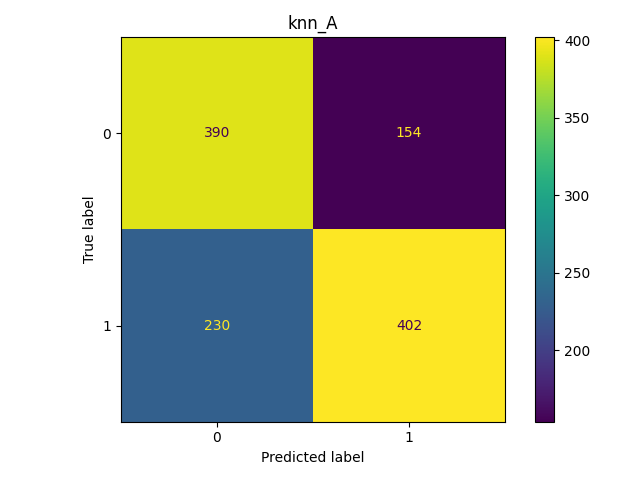
\includegraphics[width=.47\textwidth]{../results/figures/knn_A_confusion.png}\hfill
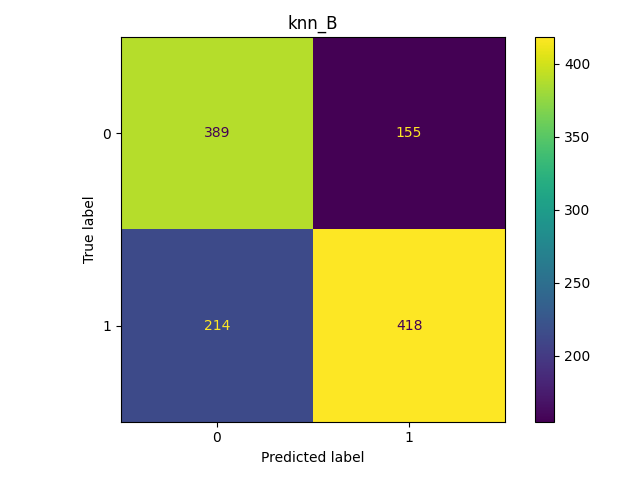
\includegraphics[width=.47\textwidth]{../results/figures/knn_B_confusion.png}
\caption{Ma trận nhầm lẫn K-NN: A bên trái và B bên phải.}\label{fig:cm-knn}
\end{figure}
Từ Hình~\ref{fig:cm-knn} và bảng số đếm, A có TN=390, FP=154, FN=230,
TP=402; B có TN=389, FP=155, FN=214, TP=418. B phát hiện thêm 16 dòng
dương nhưng tăng một FP trong tổng hợp. Những số đếm này không cho biết
đó có phải cùng các đơn hay không và không nên coi 16 dòng là 16 trường
hợp độc lập do cấu trúc nhiều mặt hàng trong đơn.

F1 train của A là 0,9994 và B là 1,0000. Khoảng cách train--CV lần lượt
0,3326 và 0,3286 rất lớn. Với trọng số distance, dự đoán trên chính các
điểm train có thể bị chi phối bởi điểm cách 0, nên F1 train cao của K-NN
không phải thước đo thuyết phục về tổng quát hóa. CV theo nhóm mới tạo
tình huống đơn chưa xuất hiện trong phần học của fold.

\subsection{Cây quyết định với A và B}
Cây A được chọn với gini, không giới hạn độ sâu và tối thiểu 20 mẫu/lá.
CV F1 là 0,6741, test F1 0,6688. Cây B cũng dùng gini và tối thiểu 20
mẫu/lá nhưng độ sâu tối đa 4; CV F1 đạt 0,7058 và test F1 0,7098.
So với A, B tăng CV F1 khoảng 0,0316 và test F1 khoảng 0,0410, đồng thời
đánh đổi Recall lấy Precision.

\begin{figure}[!htbp]\centering
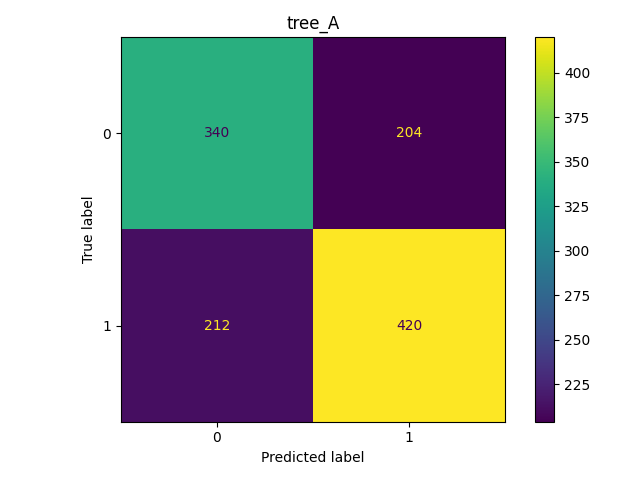
\includegraphics[width=.47\textwidth]{../results/figures/tree_A_confusion.png}\hfill
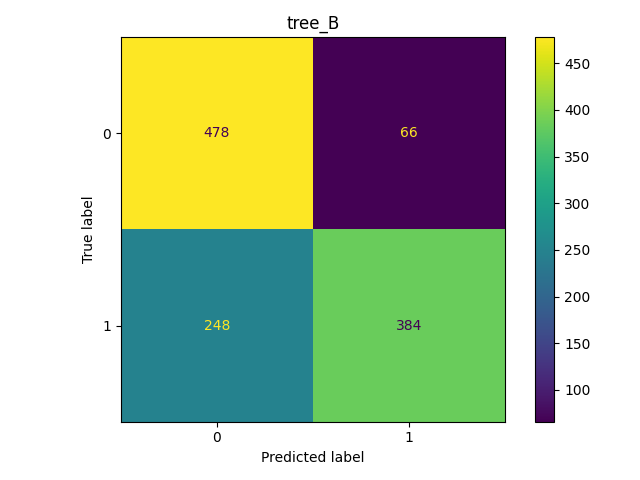
\includegraphics[width=.47\textwidth]{../results/figures/tree_B_confusion.png}
\caption{Ma trận nhầm lẫn cây A (trái) và cây B được chọn theo CV (phải).}\label{fig:cm-tree}
\end{figure}
Hình~\ref{fig:cm-tree} cho thấy cây A có TN=340, FP=204, FN=212, TP=420. Cây B có TN=478, FP=66, FN=248,
TP=384. Vì vậy, B giảm 138 FP nhưng tăng 36 FN so với A. Từ số đếm này,
không thể kết luận tổng chi phí giảm khi chưa biết giá của một cảnh báo
sai và một bỏ sót. Đây là ví dụ cụ thể cho thấy F1 cao hơn không đồng
nghĩa mọi loại lỗi đều ít hơn.

\begin{samepage}
Theo định nghĩa từ Chương~\ref{chap:2}, kiểm tra lại cây B cho
$P=384/(384+66)=0{,}8533$ và $R=384/(384+248)=0{,}6076$.
Công thức F1 theo số đếm cho $768/(768+66+248)=0{,}7098$.
Như vậy, metric trong bảng phù hợp trực tiếp với ma trận nhầm lẫn, không
lấy từ con số làm tròn trên ảnh. ROC-AUC là 0,7756 và average precision
là 0,7889; hai chỉ số không xác nhận xác suất đã hiệu chuẩn.
\par\end{samepage}

\subsection{Cross-validation, dao động và overfitting}
\begin{table}[!htbp]\centering
\caption{Mức khớp trên train, CV và chênh lệch F1 của sáu ứng viên.}\label{tab:gaps}
\begin{tabularx}{\linewidth}{Ycrrrr}\toprule
\rowcolor{reportheader} \theadcell{Mô hình} & \theadcell{Luồng} & \theadcell{Train F1} & \theadcell{CV F1} & \theadcell{SD CV} & \theadcell{Train--CV} \\\midrule
Cây cơ sở & A & 0.9994 & 0.6691 & 0.0138 & 0.3303 \\
Dummy & A & 0.6944 & 0.6944 & 0.0001 & -0.0000 \\
K-NN & A & 0.9994 & 0.6668 & 0.0060 & 0.3326 \\
Cây & A & 0.7646 & 0.6741 & 0.0154 & 0.0905 \\
K-NN & B & 1.0000 & 0.6714 & 0.0161 & 0.3286 \\
Cây & B & 0.7137 & 0.7058 & 0.0102 & 0.0079 \\
\bottomrule\end{tabularx}
\end{table}

Trong Bảng~\ref{tab:gaps}, cây B có chênh lệch train--CV nhỏ nhất trong các
mô hình dùng đặc trưng, khoảng 0,0079. Đây là dấu hiệu khả quan về mức
khớp trong protocol hiện tại. Tuy nhiên, khoảng cách nhỏ cũng có thể đi
cùng mô hình còn đơn giản và bỏ sót một nhóm lớn; kết quả Standard Class
bên dưới cho thấy không được dùng gap nhỏ để khẳng định mô hình đã đủ tốt.

Độ lệch chuẩn CV F1 của K-NN A khoảng 0,0060, K-NN B 0,0161, cây A
0,0154 và cây B 0,0102. Không gán ý nghĩa thống kê cho việc chênh lệch
trung bình lớn hay nhỏ hơn một độ lệch chuẩn. Cần repeated group split
hoặc đánh giá độc lập có thiết kế trước để đo độ ổn định. Điểm test nhỉnh
hơn CV ở một số ứng viên có thể phản ánh khác biệt độ khó của tập dữ liệu;
không chứng minh test bị dùng để huấn luyện.

Thời gian search/refit ghi nhận khoảng 41,70 giây cho K-NN A, 39,34 giây
cho K-NN B, 13,18 giây cho cây A và 19,09 giây cho cây B. Đây là chi phí
của các lưới có số cấu hình khác nhau trên một máy ở lần chạy lịch sử.
Không so sánh như benchmark tốc độ thuật toán độc lập và không suy ra
độ trễ cho từng đơn khi triển khai.

\subsection{EDA: giá trị thiếu và đặc trưng số}
\fig[.78]{02_missing.png}{Tỷ lệ thiếu trên train; chỉ thể hiện các cột thiếu nhiều nhất.}{fig:missing}
Hình~\ref{fig:missing} phản ánh cột mô tả sản phẩm thiếu hoàn toàn và mã
bưu chính đơn thiếu rất nhiều. Đây là những cột không được phép đi vào
pipeline. Hình không chứng minh rằng đầu vào mô hình đang thiếu ở mức
tương tự; Bảng~\ref{tab:missing} mô tả toàn nguồn còn hình chỉ mô tả train.
Không dùng mức thiếu ở cột bị loại để giải thích chênh lệch A/B.

\fig[.88]{03_numeric_hist.png}{Histogram bốn đặc trưng số trên train, trước scaling.}{fig:hist}
Hình~\ref{fig:hist} giúp nhận diện thang đo khác nhau giữa số ngày, số
lượng, giá và tỷ lệ chiết khấu. Những đỉnh của biến rời rạc không mặc
nhiên là bất thường; ví dụ số ngày kế hoạch và số lượng vốn có miền giá
trị hạn chế. Giá sản phẩm cần được xem xét ở thang riêng trước khi tính
khoảng cách. Đây là căn cứ phương pháp cho chuẩn hóa, chưa là thí nghiệm
chứng minh chuẩn hóa tăng bao nhiêu F1.

\fig[.78]{04_boxplot.png}{Boxplot đặc trưng số trên train với thang giá trị gốc.}{fig:box}
Do các trường chung trục gốc, trường giá có thể chiếm phần lớn chiều dài
Hình~\ref{fig:box}. Không suy ra các trường còn lại không biến thiên chỉ
vì chúng nhìn hẹp trên hình này. Báo cáo kết hợp histogram riêng và thống
kê số để tránh đọc sai tác động của thang đo. Không cắt bỏ các điểm được
đánh dấu IQR; pipeline hiện tại không có bước clipping hoặc winsorization.

\subsection{EDA: phương thức giao hàng và khu vực}
\fig[.76]{05_shipping.png}{Số dòng từng lớp theo phương thức giao hàng trên train.}{fig:shipping}
Hình~\ref{fig:shipping} đặt số đếm hai lớp cạnh nhau theo phương thức
giao. Đây là cấu trúc đáng chú ý vì cây B sau đó phân nhánh mạnh theo
Shipping Mode. Tuy nhiên, từ countplot không thể kết luận chọn phương
thức giao nhanh gây trễ: thời hạn cam kết, loại đơn và phân khúc khách
có thể khác nhau đồng thời. Cần giữ tách biệt mô tả mối liên hệ với kết
luận nhân quả.

\fig[.82]{06_regions.png}{Tỷ lệ dòng trễ theo vùng trên train, không phải số lượng đơn.}{fig:regions}
Hình~\ref{fig:regions} được đọc cùng \code{train_region_support.csv}.
Central America có 767 dòng với tỷ lệ trễ 0,5306; Western Europe 614 dòng
với 0,5326. Central Asia có tỷ lệ 0,8261 nhưng chỉ 23 dòng, trong khi
Canada có 10 dòng. Cột cao của một vùng ít quan sát không cung cấp độ
chắc chắn tương đương vùng nhiều quan sát, và các dòng còn phụ thuộc theo
đơn. Không xếp hạng chất lượng vận hành các vùng chỉ bằng hình này.

\subsection{EDA: tương quan và diễn biến theo tháng}
\fig[.73]{07_correlation.png}{Tương quan tuyến tính giữa bốn trường số trên train.}{fig:corr}
Hình~\ref{fig:corr} khảo sát quan hệ từng cặp giữa các đầu vào số, không
phải độ quan trọng mô hình. Tương quan thấp không loại trừ quan hệ phi
tuyến hoặc tương tác với phương thức giao. Ngược lại, tương quan cao
giữa hai trường cũng không tự tạo leakage nếu cả hai có sẵn ở thời điểm
dự đoán. Quyết định loại trường phải kết hợp thời điểm, ngữ nghĩa và
thiết kế thí nghiệm, không chỉ dựa hệ số tương quan.

\fig[.96]{08_month.png}{Tỷ lệ trễ theo tháng tạo đơn trên train, ghép năm--tháng.}{fig:month}
Hình~\ref{fig:month} là đường mô tả theo các khoảng năm--tháng, trong khi
đặc trưng \code{order_month} chỉ lấy tháng trong năm. Không đồng nhất hai
cách biểu diễn. Dao động trên hình gợi ý cần kiểm tra cấu trúc thời gian,
nhưng chưa chứng minh mùa vụ ổn định; số đơn mỗi tháng và thay đổi cơ cấu
đơn có thể ảnh hưởng tỷ lệ. Split nhóm ngẫu nhiên không kiểm tra khả năng
dự đoán những tháng nằm sau giai đoạn train.

\subsection{Đánh giá theo đơn và độ nhạy với đơn vị quan sát}
\begin{table}[!htbp]\centering\small
\caption{Metric theo đơn, xác suất trung bình và ngưỡng 0,5 cố định.}\label{tab:orders}
\begin{tabular}{lrrrr}\toprule
Mô hình & Accuracy & Precision & Recall & F1 \\\midrule
tree\_B & 0.7258 & 0.8554 & 0.6068 & 0.7100 \\
dummy\_A & 0.5532 & 0.5532 & 1.0000 & 0.7123 \\
\bottomrule\end{tabular}
\end{table}

Bảng~\ref{tab:orders} lấy xác suất trung bình theo 423 đơn và ngưỡng 0,5.
Tree B có TN=165, FP=24, FN=92, TP=142; Dummy có TN=0, FP=189, FN=0,
TP=234. F1 cây B theo đơn là 0,7100, gần F1 dòng 0,7098, nhưng Dummy
đạt 0,7123 và nhỉnh hơn cây B ở cấp đơn. Vì vậy, thứ tự theo F1 test có
thể phụ thuộc đơn vị tính, ngay cả khi split không đổi.

Điểm theo đơn không được dùng để chọn lại mô hình sau khi xem holdout.
Nó là chẩn đoán bổ sung về tính phù hợp với nghiệp vụ. Đơn nhiều dòng
được trọng số lớn trong metric dòng; metric đơn khắc phục cách đếm đó
nhưng cần quy tắc tổng hợp xác suất. Chưa kiểm tra quy tắc max hoặc các
ngưỡng khác; không tuyên bố trung bình là lựa chọn tối ưu.

\subsection{Ablation thời gian và phân tích lỗi theo nhóm}
\begin{table}[!htbp]\centering\small
\begin{tabular}{lrrr}\toprule
Thuật toán & A: CV F1 & B: CV F1 & B--A \\\midrule
knn & 0.6668 & 0.6714 & +0.0046 \\
tree & 0.6741 & 0.6904 & +0.0163 \\
\bottomrule\end{tabular}
\caption{Ablation lịch trên CV train với tham số của A được giữ cố định.}\label{tab:ablation}
\end{table}

Trong Bảng~\ref{tab:ablation}, cấu hình của A được cố định khi thay luồng.
K-NN tăng CV F1 khoảng 0,0046; cây tăng khoảng 0,0163. Kết quả khác với
mức tăng 0,0316 khi mỗi luồng cây tự chọn tham số riêng. Điều này cho
thấy so sánh tuned A/B trộn cả thay đổi đặc trưng lẫn lựa chọn siêu tham
số. Ablation giúp tách bớt hai yếu tố, nhưng vẫn đánh giá trên fold đã
dùng chọn tham số A nên chưa loại selection optimism.

\begin{table}[!htbp]\centering
\caption{Lỗi theo dòng của cây B, kèm mẫu số nhóm dịch vụ.}\label{tab:shipping-errors}
\begin{tabularx}{\linewidth}{Yrrrrrr}\toprule
\theadcell{Phương thức} & \theadcell{n} & \theadcell{Dương} & \theadcell{FN} & \theadcell{FP} & \theadcell{FNR} & \theadcell{FPR} \\\midrule
First Class & 203 & 193 & 0 & 10 & 0.0000 & 1.0000 \\
Same Day & 71 & 27 & 0 & 0 & 0.0000 & 0.0000 \\
Second Class & 198 & 158 & 0 & 40 & 0.0000 & 1.0000 \\
Standard Class & 704 & 254 & 248 & 16 & 0.9764 & 0.0356 \\
\bottomrule\end{tabularx}
\end{table}

\begin{samepage}
Bảng~\ref{tab:shipping-errors} ghi toàn bộ 248 FN ở Standard Class: sáu TP
trên 254 dòng dương (Recall 0,0236), 16 FP trên 450 dòng âm. First Class
có 10 FP/10 dòng âm, Second Class 40 FP/40 dòng âm. Same Day không lỗi
trên 71 dòng, chưa đủ khẳng định ổn định. Các lỗi nhóm là chẩn đoán,
không dùng để tinh chỉnh lại trên test; Chương~\ref{chap:5} phân tích giới hạn này.
\par\end{samepage}

\partstart{Thảo luận và so sánh}
\subsection{K-NN và cây quyết định trên dữ liệu hỗn hợp}
K-NN biểu diễn giả thuyết rằng các đơn gần nhau trong không gian đầu vào
có xu hướng chung nhãn. Điểm mạnh là không cần định sẵn dạng ranh giới
tuyến tính. Điểm yếu trong bài toán này là sự gần nhau phụ thuộc mạnh vào
mã hóa và thang đo. Một không gian nhiều cột one-hot có thể làm khoảng
cách khó diễn giải về nghiệp vụ; các trường địa lý hiếm còn ít láng giềng
để tham chiếu đáng tin cậy.

Cây quyết định tìm những điều kiện tách dữ liệu thành nhóm tương đối đồng
nhất. So với K-NN, đường đi qua các nút dễ đọc hơn và chi phí dự đoán trên
cây nông ít phụ thuộc số dòng train. Tuy vậy, quy tắc dễ đọc không đồng
nghĩa đúng nhân quả hay ổn định. Một split nhỏ có thể thay đổi nhánh; cây
quá sâu có thể khớp những nhóm hiếm và thể hiện khoảng cách train--CV lớn
như baseline đã quan sát.

Trong thí nghiệm, cây B vượt K-NN B về Precision và Accuracy nhưng Recall
thấp hơn. Không có thuật toán thắng toàn bộ tiêu chí. Nếu mục tiêu là
ưu tiên một danh sách ngắn có tỷ lệ đúng cao, hướng đánh đổi của cây B
đáng khảo sát thêm; nếu mục tiêu là giảm bỏ sót, Recall thấp hiện tại là
hạn chế rõ. Chưa có yêu cầu nghiệp vụ định lượng để lựa chọn giữa hai
hướng, nên báo cáo chỉ giữ tiêu chí CV F1 đã định trước.

\subsection{Ảnh hưởng quan sát được của luồng A và B}
Bổ sung lịch có lợi về F1 trong các so sánh đã lưu, nhưng mức cải thiện
khác nhau theo thuật toán và cách chọn tham số. K-NN có chênh lệch CV
0,0046, còn cây tuned có chênh lệch 0,0316. Khi giữ tham số cây A cố định,
chênh lệch chỉ 0,0163. Vì vậy, không quy toàn bộ mức tăng của cây tuned
cho ba cột thời gian; một phần so sánh đồng thời thay đổi độ sâu được chọn.

Tháng, thứ, giờ có thể là proxy cho chu kỳ vận hành, cơ cấu dịch vụ hoặc
giai đoạn thu thập dữ liệu. Đây là các khả năng giải thích cần kiểm chứng,
không phải nguyên nhân đã xác nhận. Chẳng hạn, giờ đặt đơn quan trọng trong
cây có thể phản ánh cơ chế dữ liệu riêng của Same Day thay vì một quy luật
chung cho mọi dịch vụ. Muốn kết luận cần thêm dữ liệu và thí nghiệm được
định trước, đặc biệt giữ tập tương lai độc lập.

Hai luồng không phải so sánh ``có tiền xử lý'' với ``không tiền xử lý''.
Cả hai đều có imputation, scaling và one-hot. Do đó, kết quả chỉ hỗ trợ
đối chiếu biểu diễn A với A cộng lịch, không đo riêng hiệu quả từng phép
biến đổi. Đây là giới hạn thiết kế cần nêu để tránh mô tả phương pháp
nhiều hơn bằng chứng thực sự có.

\subsection{Baseline, Dummy và ý nghĩa của F1 cạnh tranh}
Với tỷ lệ dương $\pi$ và quy tắc luôn dự đoán dương, Precision bằng $\pi$,
Recall bằng 1, nên
\begin{equation}
F_{1,\mathrm{all+}}=\frac{2\pi}{1+\pi}.
\end{equation}
Thay $\pi=632/1176$ cho test dòng thu được F1 khoảng 0,6991, đúng với
Dummy. Đây là hệ quả toán học từ số đếm lớp, không cần mô hình khai thác
đặc trưng. Vì vậy, một điểm F1 xấp xỉ 0,70 chưa tự chứng minh mô hình
phân biệt hữu ích trong bài toán này.

Cây B đạt F1 dòng cao hơn Dummy khoảng 0,0107 nhưng Precision tăng từ
0,5374 lên 0,8533, còn Recall giảm từ 1 xuống 0,6076. Đó là thay đổi
thực chất về kiểu ra quyết định. Cây chỉ cảnh báo 450/1.176 dòng, trong
khi Dummy cảnh báo toàn bộ. Tỷ lệ cảnh báo đúng cao hơn có thể giúp hạn
chế khối lượng xử lý, nhưng 248 FN vẫn là phần rủi ro lớn cần cân nhắc.

Cây baseline cho thấy một kiểu thất bại khác: gần hoàn hảo trên train
nhưng không vượt Dummy ở CV hoặc test F1. Tuned tree A cải thiện ít so
với baseline về CV và vẫn dưới Dummy. Như vậy, sử dụng thuật toán có học
không tự bảo đảm vượt đối chứng không dùng đặc trưng. Việc báo đủ baseline
là cần thiết để không trình bày metric rời bối cảnh.

\subsection{False Positive và False Negative trong nghiệp vụ}
FP là cảnh báo cho dòng được nguồn gán âm. Nó có thể dẫn tới cuộc gọi,
kiểm tra kho hoặc ưu tiên không cần thiết, nhưng dữ liệu không ghi nhận
biện pháp nào đã được thực hiện. Hơn nữa, nhãn âm còn có đơn hủy, nên
không mô tả mọi FP là ``đơn đã giao đúng hạn bị báo nhầm''. Đó là lý do
ngữ nghĩa nhãn ảnh hưởng trực tiếp tới phân tích tác động.

FN là dòng trễ không được cảnh báo. Với cây B, 248 FN trên 632 dòng dương
tương đương bỏ sót khoảng 39,24\% dòng dương toàn test. Người vận hành
không nhìn thấy các dòng này trong danh sách cảnh báo. Tuy nhiên, không
biết một can thiệp sớm có thực sự ngăn trễ hay không, nên không chuyển
số FN thành số đơn chắc chắn có thể cứu được hoặc thiệt hại tiền cụ thể.

Nếu ký hiệu chi phí một FP là $c_{FP}$ và một FN là $c_{FN}$, một mô hình
đơn giản cho tổng lỗi là $C=c_{FP}FP+c_{FN}FN$. So cây B với Dummy trên
test dòng cho
\begin{equation}
C_{B}-C_{D}=-478c_{FP}+248c_{FN}.
\end{equation}
Trong mô hình chi phí giả định này, B có chi phí thấp hơn khi
$c_{FN}/c_{FP}<478/248\approx1{,}927$, nếu $c_{FP}>0$. Đây là phép suy
ra minh họa từ số đếm đã có, không phải kết quả kinh tế được đo. Nó bỏ qua
chi phí xử lý TP, khả năng can thiệp thành công và phụ thuộc giữa các dòng.

Do nhiều dòng thuộc cùng đơn, chi phí theo dòng có thể tính lặp một hành
động. Nếu quyết định ở cấp đơn, cần dùng số FP/FN theo đơn và chi phí phù
hợp cấp đơn. Không chọn tỷ lệ chi phí sau khi thấy kết quả để chứng minh
mô hình đã tốt. Chi phí và mục tiêu Recall nên được thống nhất trước
thiết kế validation và lựa chọn ngưỡng tiếp theo.

\subsection{Standard Class là điểm yếu trọng yếu}
Standard Class chiếm 704/1.176 dòng test và chứa 254 dòng dương. Cây B
chỉ phát hiện sáu dòng dương của nhóm, bỏ sót 248. Điều này tạo nghịch lý
bề ngoài: Precision toàn mô hình cao nhưng một dịch vụ chiếm phần lớn
test gần như không được phát hiện giao trễ. Metric tổng hợp bị chi phối
bởi việc cây cảnh báo tốt ở các dịch vụ khác.

Tỷ lệ âm cao trong Standard Class khiến quy tắc phần lớn dự đoán âm có
thể đạt nhiều TN. Đây là giải thích phù hợp với số đếm và cấu trúc cây,
không khẳng định là nguyên nhân duy nhất của mọi FN. Nhãn của các đơn,
thời hạn kế hoạch và cách tạo dữ liệu có thể cùng ảnh hưởng. Không có
bằng chứng ở artifact để kết luận kho, tuyến đường hay nhân viên cụ thể
gây ra các trường hợp giao trễ này.

Ngược lại, First Class và Second Class có toàn bộ dòng âm bị cảnh báo
sai trong holdout. Hai nhóm có FPR bằng 1 nhưng mẫu số âm lần lượt chỉ
10 và 40. Báo cả tử số lẫn mẫu số giúp tránh đọc tỷ lệ như quy luật phổ
quát. Same Day không lỗi trên 71 dòng vẫn cần kiểm tra ở dữ liệu khác;
không coi số lỗi bằng 0 ở một mẫu là bằng chứng bảo đảm dịch vụ.

Một hướng nghiên cứu hợp lý là kiểm tra mô hình hoặc tiêu chí validation
có chú ý Recall từng dịch vụ. Đây là đề xuất tương lai: hiện chưa chạy
mô hình riêng Standard Class, chưa tối ưu trọng số lớp và chưa chọn
threshold theo nhóm. Những thay đổi đó cần được thiết kế, fit và lựa chọn
trên train/validation trước một test độc lập, tránh học lại từ test hiện tại.

\subsection{Diễn giải đặc trưng và quy tắc cây}
\begin{table}[!htbp]\centering
\caption{Bốn importance lớn nhất trong cây B theo artifact đã lưu.}\label{tab:importance}
\begin{tabularx}{\linewidth}{|Y|r|}\hline
\theadcell{Đặc trưng sau tiền xử lý} & \theadcell{Importance}\\\hline
Shipping Mode: Standard Class & 0,5735\\
Giờ tạo đơn & 0,1758\\
Shipping Mode: Same Day & 0,1356\\
Shipping Mode: First Class & 0,0624\\\hline
\end{tabularx}

\end{table}
Bảng~\ref{tab:importance} cho thấy phần lớn mức giảm impurity gắn với
Shipping Mode và giờ tạo đơn. Quy tắc xuất bắt đầu bằng chỉ báo Standard
Class, sau đó có các nhánh Same Day và địa lý. Điều này phù hợp với sự
khác nhau rõ về hành vi dự đoán giữa nhóm dịch vụ. Importance thuộc từng
cột one-hot, không phải phép đo nhân quả của toàn trường gốc.

Một phần quy tắc thực trong \code{tree_B_rules.txt} là nhánh Same Day
so sánh \code{numeric__order_hour <= 0.03}. Giá trị 0,03 nằm trên thang
StandardScaler, không phải 0,03 giờ trong ngày. Muốn chuyển về giờ gốc
cần dùng $x=\mu+s z$ với tham số scaler đã fit của đúng mô hình. Báo cáo
không có đủ các tham số đó trong bảng aggregate để tự thay ngưỡng bằng
một giờ cụ thể.

Các nhánh có thể chứa điều kiện khác nhau nhưng kết thúc cùng nhãn 1.
Điều đó không có nghĩa điều kiện hoàn toàn vô dụng: phân bố xác suất ở
lá có thể khác dù argmax giống nhau. Ngược lại, chỉ xem nhãn ở cây xuất
không đủ để khẳng định xác suất chính xác. Muốn dùng xác suất làm ưu tiên
cần kiểm tra calibration và độ ổn định ở dữ liệu độc lập.

\subsection{Đánh giá cấp dòng và cấp đơn}
Metric dòng trả lời hiệu quả trên một dòng hàng được chọn theo phân phối
test. Metric đơn trả lời hiệu quả khi mỗi đơn có trọng số ngang nhau.
Nếu đơn nhiều mặt hàng gặp cùng lỗi, metric dòng có thể khuếch đại trọng
số của tình huống đó. Chia nhóm giải quyết việc rò rỉ giữa hai tập, nhưng
không tự thay đổi trọng số metric từ dòng sang đơn.

Trên 423 đơn, cây B có Precision 0,8554, Recall 0,6068 và F1 0,7100;
Dummy F1 0,7123. Mức chênh nhỏ và thứ tự đảo so với F1 dòng làm rõ việc
chọn đơn vị đánh giá phải gắn với đơn vị hành động. Không thay tiêu chí
chọn mô hình sau khi nhìn thấy sự đảo thứ tự. Trong nghiên cứu tiếp theo,
nếu sản phẩm cảnh báo theo đơn thì metric validation cũng nên được xác
định ở cấp đơn ngay từ đầu.

Quy tắc trung bình xác suất giả định mọi dòng của đơn có vai trò ngang
nhau. Một mặt hàng đặc biệt có thể cần cách tổng hợp khác, nhưng dataset
không cung cấp mục tiêu hành động đủ rõ để chọn quy tắc mới. Không suy
ra trung bình tốt hơn max hoặc ngược lại khi chưa có thí nghiệm. Phân
tích hiện tại chỉ kiểm tra một cách tổng hợp đã được lưu trong protocol.

\subsection{Tính đại diện, giới hạn dữ liệu và tổng quát hóa}
Mẫu 2.113 đơn là phần nhỏ trong 65.752 đơn nguồn. Kiểm tra sampling ghi
nhận chênh lệch tỷ lệ biên lớn nhất khoảng 0,0227 ở Customer Segment
trong các danh mục đã khảo sát. Sự gần nhau của một số tỷ lệ không bảo
đảm quan hệ giữa phương thức giao, vùng, thời gian và nhãn cũng giống
nhau. Các tổ hợp hiếm có thể còn rất ít hoặc vắng trong mẫu.

Cách chọn tiền tố sau xáo trộn nhóm giữ nguyên đơn nhưng vẫn chịu ràng
buộc kích thước nhóm và ngân sách. Không gọi nó là mẫu phân tầng theo
mọi trường hoặc mẫu không chệch đã chứng minh. Một seed duy nhất không
đo độ nhạy kết quả với việc đơn nào được đưa vào. Lặp lấy mẫu theo nhóm
có thể cung cấp phân phối metric, nhưng chưa được thực hiện ở đây.

Nguồn lịch sử còn có khác biệt giữa nhãn giao trễ và trạng thái hủy,
giới hạn về cách ghi timestamp, danh mục địa lý và thời điểm một số trường
được hình thành. Không có kiểm chứng vận hành để xác nhận các quan hệ
quan sát được sẽ giữ nguyên ở doanh nghiệp khác. Vì vậy, không dùng từ
``tổng quát tốt'' chỉ dựa trên một holdout nhóm ngẫu nhiên.

\subsection{Khả năng ứng dụng và những hạn chế còn lại}
Ở trạng thái hiện tại, sản phẩm phù hợp làm nghiên cứu học phần và bằng
chứng cho quy trình có kiểm soát. Một ứng dụng thử nghiệm hợp lý trong
tương lai là chạy song song với quy trình hiện hữu, chỉ ghi cảnh báo để
đo chất lượng mà chưa tự điều phối. Cần thống nhất thời điểm chấm điểm,
đơn vị đơn hàng, định nghĩa trễ và mục tiêu phát hiện trước khi triển khai.

Các điều kiện còn thiếu gồm kiểm định thời gian, dữ liệu vận hành độc
lập, chi phí lỗi, hiệu chuẩn xác suất, khoảng tin cậy theo nhóm và giám
sát drift. Ngoài ra, nhóm cần xác nhận tính sẵn có của thuộc tính ngay
tại lúc tạo đơn. Một mô hình chạy đúng pipeline nhưng dùng cột xuất hiện
muộn hơn giả định vẫn không đáp ứng bài toán cảnh báo sớm.

Không có kết quả nào trong báo cáo chứng minh cảnh báo giúp giảm tỷ lệ
giao trễ thực tế. Để kiểm tra điều đó cần thiết kế đo tác động can thiệp,
khác với bài toán đo dự đoán. Việc giữ ranh giới giữa hiệu quả phân loại
và hiệu quả điều hành giúp các hướng phát triển có tiêu chí kiểm chứng
rõ ràng, thay vì chỉ đặt mục tiêu nâng thêm vài phần trăm F1.

\partstart{Tổng kết và hướng phát triển}
\subsection{Các mục tiêu đã thực hiện}
Đề tài đã xây dựng quy trình phân loại nguy cơ giao trễ trên DataCo,
có kiểm toán schema, nhãn, missing, outlier và cấu trúc đơn nhiều dòng.
Allowlist loại các trường kết quả và định danh; chia train/test và CV
theo mã đơn hạn chế rò rỉ giữa các dòng chung đơn.

K-NN và cây quyết định được so sánh trên A/B với cây mặc định và Dummy.
Mô hình được chọn bằng F1 CV; tiền xử lý fit trong từng fold, test chỉ
đánh giá sau khi khóa lựa chọn. Cấu hình, hash, phiên bản, bảng và hình
được lưu để truy vết.

Ma trận nhầm lẫn, khoảng cách train--CV, ablation lịch, metric theo đơn
và lỗi theo dịch vụ bổ sung cho đánh giá tổng thể, chỉ ra điểm yếu
Standard Class thay vì chỉ xếp hạng thuật toán.

\subsection{Kết quả chính và mức độ kết luận}
Trên mẫu 5.999 dòng, cây B được chọn với độ sâu 4, tối thiểu 20 mẫu/lá,
gini và ba đặc trưng lịch bổ sung. CV F1 đạt 0,7058, test F1 theo dòng
0,7098; Precision 0,8533 và Recall 0,6076. Các giá trị này mô tả kết quả
của đúng một protocol và một tập con, không phải đánh giá trên toàn bộ
180.519 dòng hay một dữ liệu ngoài độc lập.

K-NN B cải thiện so với A trong kết quả đã lưu, nhưng F1 train gần 1 và
CV thấp hơn đáng kể cho thấy cần thận trọng về tổng quát hóa. Cây baseline
cũng có khoảng cách train--CV lớn. Cây B nông có gap nhỏ hơn, song bỏ sót
248/254 dòng dương Standard Class. Vì vậy, cải thiện về kiểm soát độ phức
tạp chưa giải quyết được thất bại ở nhóm dịch vụ này.

Dummy đạt F1 dòng 0,6991 và F1 đơn 0,7123 bằng cách dự đoán mọi trường
hợp dương. Cây B đạt F1 đơn 0,7100, với Precision cao hơn nhưng Recall
thấp hơn nhiều. Kết quả nhấn mạnh cần đánh giá baseline và đơn vị nghiệp
vụ ngay từ thiết kế, thay vì coi một ngưỡng F1 tuyệt đối là đủ để kết
luận mô hình tốt. Hiện chưa có bằng chứng đủ để khuyến nghị tự động ra
quyết định vận chuyển.

\subsection{Điểm mạnh và hạn chế của quy trình}
Điểm mạnh là kiểm soát rò rỉ ở nhiều tầng: đặc trưng, nhóm và nơi fit
tiền xử lý. Sự nhất quán giữa cấu hình, runner và notebook giúp giảm sai
khác protocol. Manifest và artifact tổng hợp tạo đường truy vết từ số
liệu đến bảng/hình báo cáo. Các ví dụ lỗi được lọc thông tin cá nhân,
trong khi dữ liệu thô và model cục bộ không cần đưa vào bản công bố.

Hạn chế quan trọng của dữ liệu là nhãn âm chứa đơn hủy, thời điểm nghiệp
vụ của một số cột chưa có xác nhận độc lập và nguồn có thể không đại diện
cho vận hành tương lai. Hạn chế thực nghiệm là lấy một mẫu nhỏ, một seed,
ba fold và một holdout nhóm ngẫu nhiên. Chưa có khoảng tin cậy theo đơn,
đánh giá ngoài thời gian hoặc trên doanh nghiệp khác.

Hạn chế mô hình gồm khoảng cách phụ thuộc mã hóa ở K-NN, cây nhạy với
mẫu và nhóm hiếm, xác suất chưa hiệu chuẩn và các ngưỡng chưa gắn chi
phí. Không gian tìm kiếm nhỏ cũng giới hạn phạm vi kết luận về siêu
tham số. Những điểm chưa thực hiện không được mô tả như tính năng đã
có hoặc như kết quả chắc chắn sẽ cải thiện.

\subsection{Lộ trình phát triển có thể kiểm chứng}
Ưu tiên đầu tiên là làm rõ hợp đồng dữ liệu: định nghĩa đơn bị trễ,
cách xử lý đơn hủy, múi giờ và thời điểm có từng thuộc tính. Nếu thay
nhãn hoặc quần thể, cần lưu phiên bản dữ liệu và protocol mới, không
ghép trực tiếp metric cũ với metric mới. Việc xác nhận này quyết định
mô hình đang giải đúng bài toán nghiệp vụ hay chỉ khớp nhãn trong CSV.

Ưu tiên thứ hai là đánh giá tổng quát hóa. Có thể mở rộng mẫu theo ngân
sách, lặp group split với nhiều seed và bổ sung temporal holdout được
giữ độc lập. Kết quả nên có khoảng tin cậy bootstrap theo đơn; các dòng
trong cùng đơn phải đi cùng nhau ở mỗi lần resample. Nếu mục tiêu phục
vụ khách mới, cần thêm thiết kế tách khách hàng thay vì chỉ tách đơn.

Ưu tiên thứ ba là thiết kế tiêu chí vận hành. Cần xác định mức Recall
tối thiểu, số cảnh báo có thể xử lý và chi phí FP/FN. Threshold hoặc
calibration chỉ được học trên validation, không dùng test hiện tại.
Recall Standard Class cần được theo dõi riêng để tránh mô hình cải
thiện điểm trung bình nhưng tiếp tục bỏ sót một nhóm lớn.

Sau cùng mới cân nhắc mở rộng biểu diễn hoặc mô hình: mã hóa chu kỳ
cho biến lịch, đặc trưng vận hành có thời điểm rõ ràng, hay các cấu hình
kiểm soát lớp và độ phức tạp. Mọi phương án cần đối chứng cùng protocol
và có ngân sách tính toán ghi rõ. Không mặc định thêm mô hình phức tạp
sẽ vượt baseline hoặc giải được điểm yếu Standard Class.

\subsection{Điều kiện ứng dụng thực tế}
Nếu các bước trên đạt yêu cầu, hệ thống có thể được thử ở chế độ chỉ
ghi nhận, theo dõi schema, tỷ lệ danh mục lạ, phân phối xác suất và metric
khi nhãn hoàn thiện. Việc đánh giá cần tính độ trễ xuất hiện nhãn, vì
chưa giao xong không đồng nghĩa không trễ. Một cơ chế ghi nhật ký giúp
phân biệt thay đổi mô hình với thay đổi cách vận hành.

Để chứng minh lợi ích thực tế, cần đo thêm tác động của quy trình xử lý
cảnh báo, không chỉ F1. Tỷ lệ cảnh báo đúng, thời gian nhân viên xử lý
và kết quả sau can thiệp phải được thu thập theo kế hoạch phù hợp. Trong
phạm vi hiện tại, đóng góp của đề tài là một quy trình có thể kiểm tra,
các kết quả thực nghiệm được truy vết và nhận diện rõ giới hạn cần
khắc phục trước khi mở rộng.

\clearpage\phantomsection
\addcontentsline{toc}{section}{TÀI LIỆU THAM KHẢO}
\setlength{\bibhang}{1.27cm}
\setlength{\bibsep}{6pt}
\begin{thebibliography}{9}
\raggedright
\bibitem[Constante(2019)]{dataco}
Constante, F. (2019). \textit{DataCo SMART SUPPLY CHAIN FOR BIG DATA ANALYSIS} (Version 5) [Data set]. Mendeley Data. \url{https://doi.org/10.17632/8gx2fvg2k6.5}

\bibitem[Lê Thị Thùy Trang(n.d.)]{fit}
Lê Thị Thùy Trang. (n.d.). \textit{Hướng dẫn thực hiện bài tập lớn học phần Nhập môn Học máy} [Tài liệu học phần, năm học 2026–2027]. \url{https://drive.google.com/file/d/1CW72dalb1s9FCoNGUwssmFAtvp0yRNi-/view}

\bibitem[scikit-learn developers(n.d.-a)]{pitfalls}
scikit-learn developers. (n.d.-a). \textit{Common pitfalls and recommended practices}. scikit-learn. Truy cập ngày 17 tháng 11 năm 2026, từ \url{https://scikit-learn.org/stable/common_pitfalls.html}

\bibitem[scikit-learn developers(n.d.-b)]{cv}
scikit-learn developers. (n.d.-b). \textit{Cross-validation: Evaluating estimator performance}. scikit-learn. Truy cập ngày 17 tháng 11 năm 2026, từ \url{https://scikit-learn.org/stable/modules/cross_validation.html}

\bibitem[scikit-learn developers(n.d.-c)]{tree}
scikit-learn developers. (n.d.-c). \textit{Decision trees}. scikit-learn. Truy cập ngày 17 tháng 11 năm 2026, từ \url{https://scikit-learn.org/stable/modules/tree.html}

\bibitem[scikit-learn developers(n.d.-d)]{metrics}
scikit-learn developers. (n.d.-d). \textit{Metrics and scoring: Quantifying the quality of predictions}. scikit-learn. Truy cập ngày 17 tháng 11 năm 2026, từ \url{https://scikit-learn.org/stable/modules/model_evaluation.html}

\bibitem[scikit-learn developers(n.d.-e)]{knn}
scikit-learn developers. (n.d.-e). \textit{Nearest neighbors}. scikit-learn. Truy cập ngày 17 tháng 11 năm 2026, từ \url{https://scikit-learn.org/stable/modules/neighbors.html}

\bibitem[Tiwari(n.d.)]{kaggle}
Tiwari, S. (n.d.). \textit{DataCo SMART SUPPLY CHAIN FOR BIG DATA ANALYSIS} [Data set]. Kaggle. \url{https://www.kaggle.com/datasets/shashwatwork/dataco-smart-supply-chain-for-big-data-analysis}
\end{thebibliography}

\end{document}
